\chapter{Априорные распределения параметров смеси экспертов}

Данный раздел посвящен анализу свойств смеси экспертов. Рассматриваются различные способы выбора априорного распределения. Анализируется случай, когда выбраны как информативное так и неинформативное априорные распределения параметров каждого эксперта. Экспертами назначаются линейные модели. Смесь экспертов это комбинация экспертов при помощи шлюзовой функции. Рассматривается задача поиска окружностей на изображении. Каждой окружности на изображении соответствует свой эксперт. Рассматривается два случая с зависимыми и независимыми априорными распределениями параметрами локальных моделей~--- экспертов. Требуется найти на изображении синтетически сгенерированные окружности с разным уровнем шума. Сравнивается устойчивость к шуму смеси с заданными априорными распределениями на вектора параметров экспертов и без задания априорного распределения.

\begin{figure}[h!t]\center
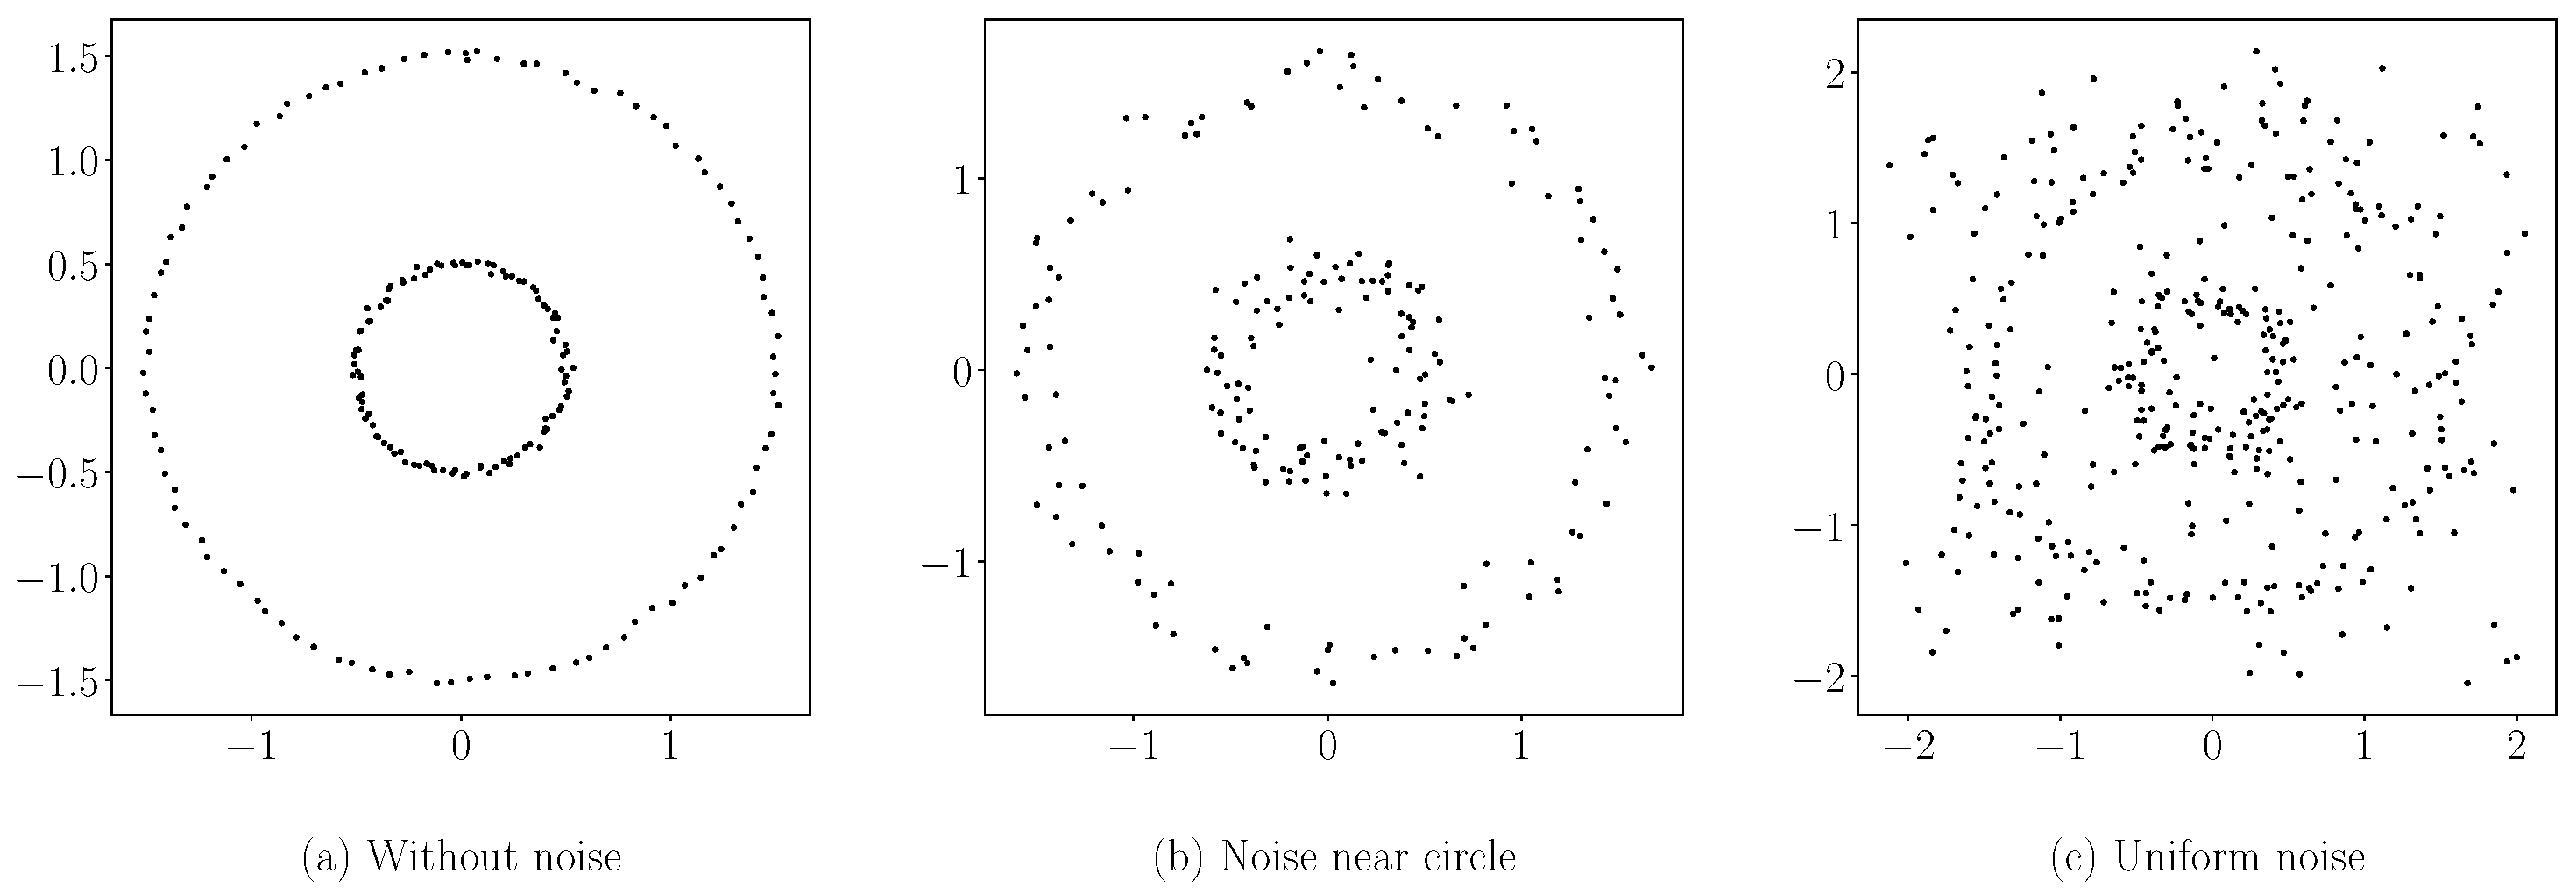
\includegraphics[width=1\textwidth]{results/priorexpert/statment}
\caption{Пример окружностей с разным уровнем шума: (a) окружности без шума; (b) окружности с зашумленным радиусом; (c) окружности с зашумленным радиусом, а также с равномерным шумом по всему изображению}
\label{example-exp:1}
\end{figure}

В рамках данной главы решается задача поиска окружностей на бинаризованном изображении. Предполагается, что радиусы окружностей различаются значимо, а также, что центры почти совпадают. Пример изображений показан на рис. \ref{example-exp:1}. В качестве экспертов рассматриваются линейные модели --- каждая модель аппроксимирует одну окружности. В качестве шлюзовой функции рассматривается двухслойная нейронная сеть.

Предлагается метод \textit{обучения с экспертом}, который предполагает использование предметных знаний экспертов для улучшения качества аппроксимации, а также для получения интерпретируемых моделей машинного обучения.
Предметные знания экспертов об образце будут называться \textit{экспертная информация}.
Предполагается, что использование экспертной информации позволяет аппроксимировать выборку простыми интерпретируемыми моделями, такими как линейные модели. Методы машинного обучения, которые учитывают экспертные знания при построении моделей, называются \textit{экспертным обучением}.

Решается задача аппроксимации кривых второго порядка на контурном изображении. Кривые второго порядка выбираются для анализа, так как они легко описываются линейными моделями. В этом случае эти фигуры необходимо восстанавливать в таких прикладных задачах, как задача распознавания радужной оболочки глаза~\cite{Matveev2010,Matveev2014,Bowyer2010}, задача описания трека частицы в адронный коллайдер~\cite{Dalila2018}. Экспертная информация о кривой второго порядка позволяет отображать точки на плоскости в новое описание объекта, где каждая кривая аппроксимируется одной линейной моделью. Модель аппроксимирующая одну кривую, называется \textit{локальной моделью}. Для аппроксимации всего контурного изображения необходимо аппроксимировать несколько кривых второго порядка с помощью нескольких локальных моделей. Вводятся ограничения на изображения: а) изображение состоит только из кривых второго порядка; б) изображение аппроксимируется небольшим количеством кривых второго порядка; в) количество и тип кривых на изображении известны.

\begin{figure}[h!]
\center
     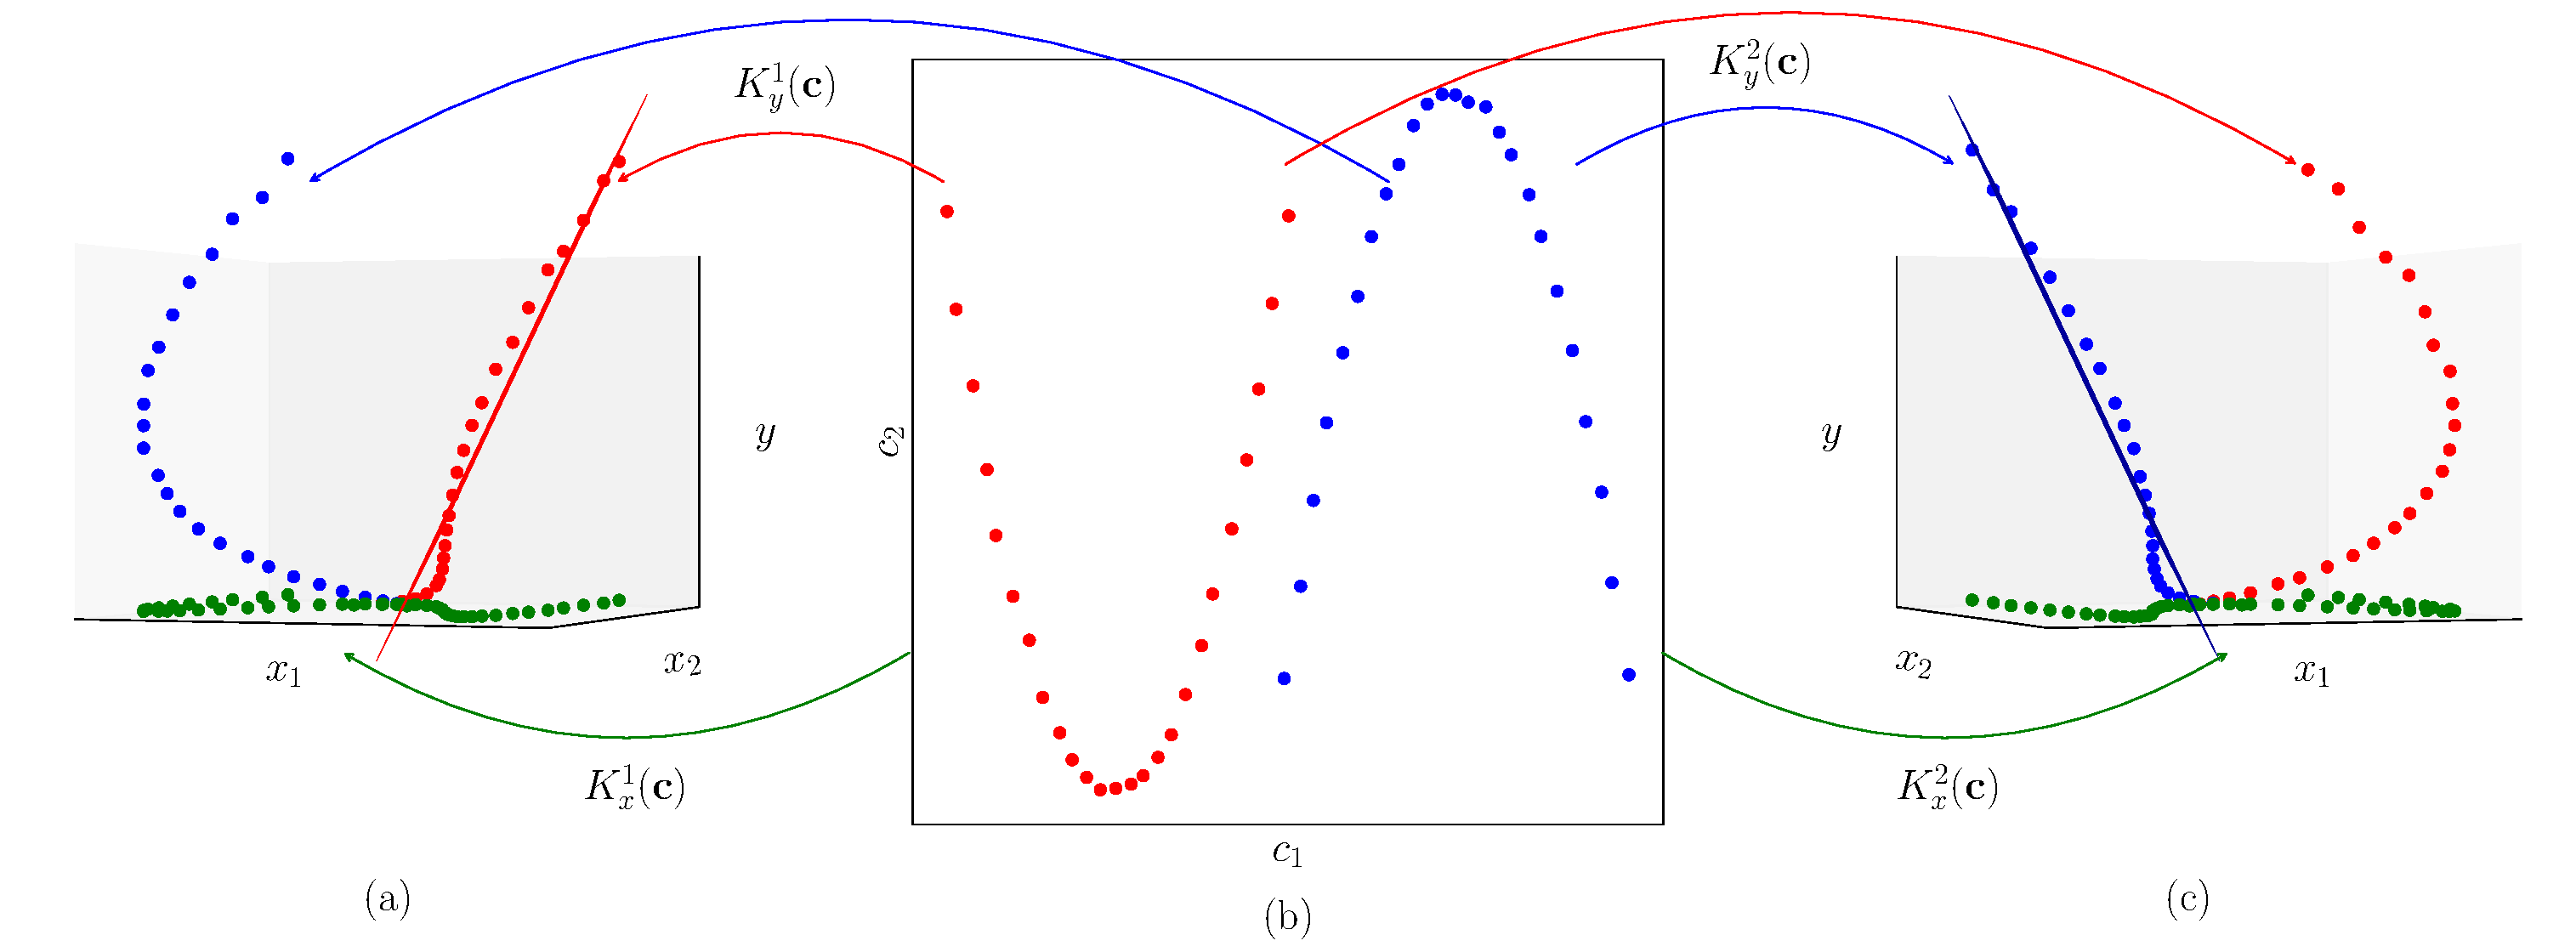
\includegraphics[width=\textwidth]{results/priorexpertfig/explanation}
     \caption{Пример: а) экспертная информация первого эксперта; б) исходные данные; в) экспертная информация второго эксперта}
    \label{intro:fig2}
\end{figure}
На рисунке \ref{intro:fig2} показан пример кривых второго порядка, а также экспертная информация о кривых. На рисунке \ref{intro:fig2}.a показана экспертная информация первого эксперта. Используя эту информацию, первая кривая аппроксимируется линейной моделью, а вторая кривая~--- шумом. На рисунке \ref{intro:fig2}.b показана экспертная информация второго эксперта. Используя эту информацию, вторая кривая аппроксимируется линейной моделью, а первая кривая представляет собой шум.

Основной проблемой построения мультимоделей является то, что мультимодель зависит от начальной инициализации параметров локальных моделей. Для повышения устойчивости мультимодели предлагается использовать вероятностную постановку задачи для поиска оптимальных параметров шлюзовой функции и параметров локальной модели. Предлагается задать априорное распределения на параметры локальных моделей, также, для повышения предлагается учесть зависимость априорных распределений для разных моделей.

При аппроксимации нескольких кривых на одном контурном изображении строится мультимодель. Примером нескольких моделей является случайный лес~\cite{Ishwaran2012}, бустинг деревьев~\cite{Chunyan2016}, смесь экспертов~\cite{Yuksel2012}. В данной работе смесь экспертов рассматривается как мультимодель. Смесь экспертов~--- это мультимодель, которая линейно взвешивает локальные модели аппроксимирующие часть выборки. Значения весовых коэффициентов зависят от объекта, для которого делается прогноз. Для решения проблемы смеси  экспертов используется вариационный EM-алгоритм~\cite{Dempster1977,bishop2006,Peng1996}.

В качестве примера рассматривается задача аппроксимации изображения радужной оболочки глаза. На рисунке \ref{intro:fig1:real} показан пример изображения для аппроксимации. Рассматриваем обработанное изображение, которое дано в виде схемы, пример такого изображения показан на рисунке \ref{intro:fig1:outer}. На рисунке \ref{intro:fig1:outer} показаны две модели окружностей, которые аппроксимируют радужную оболочку глаза. Окружности~--- простой пример кривой второго порядка.

\begin{figure}[h!]
\center
	\subfloat[]{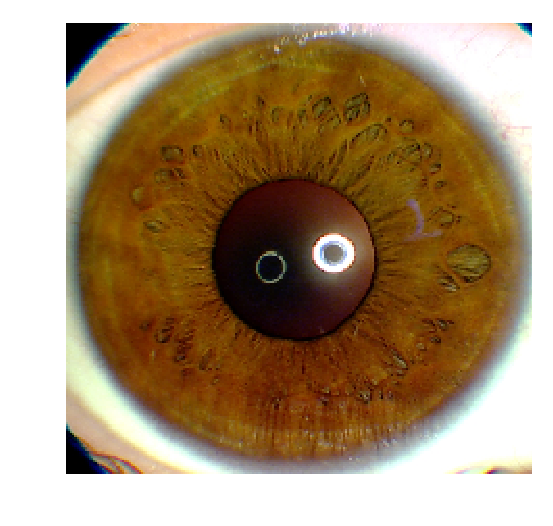
\includegraphics[height = 0.2\textheight]{results/priorexpertfig/real_image}\label{intro:fig1:real}} 
	\subfloat[]{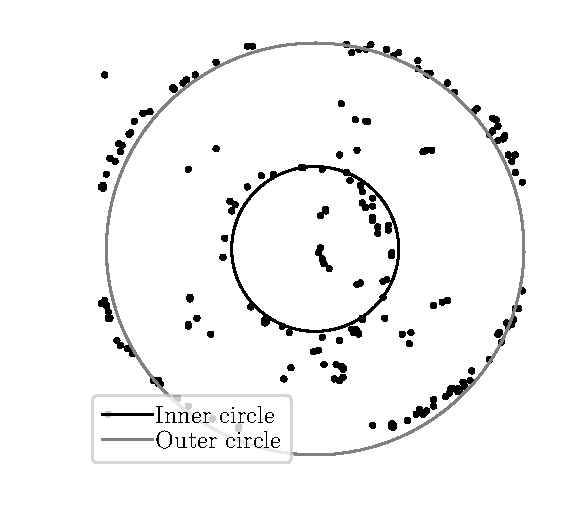
\includegraphics[height = 0.2\textheight]{results/priorexpertfig/outline_image}\label{intro:fig1:outer}} 
\caption{Пример изображения радужной оболочки глаза и ее контурное изображение: а) изображение радужной оболочки глаза; б) контурное изображение радужной оболочки и аппроксимация заданного изображения окружностей}
\label{intro:fig1}
\end{figure}

Для задачи аппроксимации радужной оболочки глаза используется экспертная информация: радужная оболочка глаза аппроксимируется двумя концентрическими окружностями. Экспертная информация используется для построения описания характеристик точек на плоскости, а также для построения функции оптимизации. Часть функции ошибок для оптимизации, использующая экспертную информацию, называется регуляризатором. Таким образом, информация о том, что изображение окружностей задается описанием признака, и информация о том, что концентрические окружности задаются с помощью специального регуляризатора.

В вычислительном эксперименте качество аппроксимации контурного изображения анализируется в зависимости от заданной экспертной информации и от уровня шума в синтетически сгенерированных данных. Анализ качества аппроксимации диафрагмы проводится в зависимости от количества экспертной информации, которая использовалась при построении модели. Важно, что каждое изображение представляет собой отдельный набор точек, которые необходимо аппроксимировать.

\section{Локальные модели в задаче построения смеси экспертов}
Задано бинарное изображение
\[
\label{ch4-eq:st:cr:1}
\begin{aligned}
\textbf{M} \in \{0,1\}^{m_1 \times m_2},
\end{aligned}
\]
где~$1$ --- это черный пиксель, который принадлежит рассматриваемой фигуре на изображении, а~$0$ --- белый пиксель, который является фоном изображения. 
Пример изображения показан на рис. \ref{example:1}.
Изображение~$\textbf{M}$ отображается в множество координат \mbox{$\textbf{C}=\left\{x_i, y_i\right\}_{i=1}^{N}$}. Координата~$(x_i, y_i)$ является координатой~$i$-го черного пикселя на изображении~$\textbf{M}$:
\[
\label{ch4-eq:st:cr:2}
\begin{aligned}
\textbf{C} \in  \mathbb{R}^{N \times 2},
\end{aligned}
\]
где~$N$~--- число черных пикселей.

Обозначим точку~$(x_0, y_0)$ центром окружности, а~$r$ радиусом окружности.
Координаты~$\left(x_i, y_i\right)\in\textbf{C}$ это геометрическое место точек, которое удовлетворяет системе уравнений:
\[
\label{ch4-eq:st:cr:3}
\begin{aligned}
\bigr(x_i - x_0\bigr)^{2}+\bigr(y_i-y_0\bigr)^2 = r^2 + \varepsilon_i, \qquad \forall i \in \{1, \ldots, N\},
\end{aligned}
\]
где~$\varepsilon_i \in \mathcal{N}\bigr(0, \beta^{-1}\bigr)$ является невязкой~$i$-го уравнения, которая является следствием шума на изображении.

Раскрыв скобки получаем
\[
\label{ch4-eq:st:cr:4}
\begin{aligned}
\left(2x_0\right)\cdot x_i + \left(2y_0\right)\cdot y_i+\left(r^2-x_0^2-y_0^2\right)\cdot1 = x_{i}^2 + y_{i}^2 + \varepsilon_i.
\end{aligned}
\]
Выражение \eqref{ch4-eq:st:cr:4} является задачей линейной регрессии с параметрами:
\[
\label{ch4-eq:st:cr:5}
\begin{aligned}
\hat{\textbf{w}} = \arg\min_{\textbf{w}\in \mathbf{R}^{n}}||\textbf{X}\textbf{w} - \textbf{y}||,  \quad \textbf{X} = \left[\textbf{C}, \textbf{1}\right], \quad \textbf{y} = \left[x_1^2+y_1^2, x_2^2+y_2^2, \ldots, x_N^2+y_N^2\right]^{\mathsf{T}}.
\end{aligned}
\]
Используя вектор параметров~$\hat{\textbf{w}} = \left[w_1, w_2, w_3\right]^{\mathsf{T}}$ получим параметры окружности~$x_0, y_0, r$:
\[
\label{ch4-eq:st:cr:6}
\begin{aligned}
x_0 = \frac{w_1}{2}, \quad y_0 = \frac{w_2}{2}, \quad r = \sqrt[]{w_3+x_{0}^{2}+y_{0}^{2}}.
\end{aligned}
\]
Решение уравнения \eqref{ch4-eq:st:cr:5} находит параметры единственной окружности на изображении. В случае, когда на изображении несколько окружностей, предлагается использовать смесь экспертов, которая состоит из линейных модели~--- экспертов. Каждый эксперт описывает одну окружность на изображении.

Обобщим подход аппроксимации одной окружности на изображении на случай, когда на изображении несколько окружностей. Пусть изображение состоит из~$K$ окружностей, тогда множество черных пикселей~$\textbf{C}$ представляется в виде:
\[
\label{ch4-eq:st:1}
\begin{aligned}
\textbf{C} = \sqcup_{k=1}^{K}\textbf{C}_{k}',
\end{aligned}
\]
где~$\textbf{C}_{k}'$ множество точек принадлежащих~$k$-й окружности. Множеству точек~$\textbf{C}_{k}' \subset\textbf{C}$ соответсвует задача линейной регрессии для выборки~$\textbf{X}_{k}' \subset \textbf{X}, \textbf{y}_{k}' \subset \textbf{y}$. Модель~$\mathbf{g}_k$ аппроксимирующая выборку~$\textbf{X}_{k}', \textbf{y}_{k}'$ является локальной моделью для выборки \textbf{X}, \textbf{y}.


\begin{definition}
\label{def:1}
Модель~$\mathbf{g}$ называется локальной моделью для выборки~$\textbf{U},$ если~$\mathbf{g}$ аппроксимирует некоторое не пустое подмножество~$\textbf{U}'\subset\textbf{U}$.
\end{definition}

\begin{definition}
\label{def:2}
Мультимодель~$\mathbf{f}$ называется смесью экспертов, если
\[
\label{ch4-eq:st:2}
\begin{aligned}
\mathbf{f} = \sum_{k=1}^{K}\pi_{k}\mathbf{g}_k\bigr(\mathbf{w}_k\bigr), \qquad \pi_{k}\bigr(\mathbf{x}, \mathbf{V}\bigr):\mathbb{R}^{n\times \left|\mathbf{V}\right|} \to [0, 1], \qquad \sum_{k=1}^{K}\pi_{k}\bigr(\mathbf{x}, \mathbf{V}\bigr) = 1,
\end{aligned}
\]
где~$\mathbf{g}_k$ является~$k$-й локальной моделью,~$\pi_k$ --- шлюзовая функция, вектор~$\mathbf{w}_k$ является параметрами~$k$-й локальной моделью, а~$\mathbf{V}$ --- параметры шлюзовой функции.
\end{definition}

В качестве локальных моделей рассматриваются линейные модели. В качестве шлюзовой функции рассматривается двухслойный перцептрон:
\[
\label{ch4-eq:st:3}
\begin{aligned}
\mathbf{g}_k\bigr(\textbf{x}\bigr) = \textbf{w}_k^{\mathsf{T}}\textbf{x}, \quad
\bm{\pi}\bigr(\mathbf{x}, \mathbf{V}\bigr) = \text{softmax}\bigr(\mathbf{V}_{1}^{\mathsf{T}}\bm{\sigma}\bigr(\mathbf{V}_2^{\mathsf{T}}\mathbf{x}\bigr)\bigr),
\end{aligned}
\]
где~$\mathbf{V} = \bigr\{\mathbf{V}_1, \mathbf{V}_2\bigr\}$~--- множество параметров шлюзовой функции.

Предлагается использовать вероятностный подход для описания смеси экспертов. Вводиться предположение, что~$\textbf{y}$ является случайным вектором, который задается плотностью распределения~$p\bigr(\textbf{y}|\textbf{X}\bigr)$. Предполагается, что плотность распределения~$p\bigr(\textbf{y}|\textbf{X}, \textbf{f}\bigr)$ аппроксимирует истинную плотность распределения~$p\bigr(\textbf{y}|\textbf{X}\bigr)$:
\[
\label{ch4-eq:st:new:1}
\begin{aligned}
p\bigr(\textbf{y}|\textbf{X}, \textbf{f}\bigr) = \prod_{i=1}^{N}\left(\sum_{k=1}^{K}\pi_kp_{k}\bigr(y_{i}|\textbf{g}_{k}\bigr(\mathbf{x}_{i}\bigr)\bigr)\right),
\end{aligned}
\]
где~$\textbf{f}$~--- это смесь экспертов, а~$\textbf{g}_k, \bm{\pi}$ определяются выражением \eqref{ch4-eq:st:3}.

Пусть~$\textbf{w}_k$ является случайным вектором, который задается плотностью распределения~$p^{k}\bigr(\mathbf{w}_k\bigr)$. Получим совместное распределения параметров локальных моделей и вектора ответов:
\[
\label{ch4-eq:st:4}
\begin{aligned}
p\bigr(\mathbf{y}, \mathbf{W}|\mathbf{X}, \mathbf{V}\bigr) = \prod_{k=1}^{K}p^{k}\bigr(\mathbf{w}_k\bigr)\prod_{i=1}^{N}\left(\sum_{k=1}^{K}\pi_{k}p_{k}\bigr(y_i|\mathbf{w}_k, \mathbf{x}_i\bigr)\right),
\end{aligned}
\]
где~$\mathbf{W} = \bigr\{\mathbf{w}_1, \mathbf{w}_2, \ldots, \mathbf{w}_K\bigr\}.$
Оптимальные параметры находятся при помощи максимизации правдоподобия:
\[
\label{ch4-eq:st:5}
\begin{aligned}
\hat{\mathbf{V}}, \hat{ \mathbf{W}} = \arg\max_{\mathbf{V}, \mathbf{W}} p\bigr(\mathbf{y},  \mathbf{W}|\mathbf{X}, \mathbf{V}\bigr).
\end{aligned}
\]

\section{Вероятностное обоснование смеси экспертов}
Для построения смеси экспертов (\ref{ch4-eq:st:2},  \ref{ch4-eq:st:4}), введем вероятностные предположения о данных \eqref{ch4-eq:st:cr:5}:

\begin{enumerate}[1)]
	\item правдоподобие~$p_{k}\bigr(y_{i}|\mathbf{w}_{k}, \mathbf{x}_{i}\bigr) = \mathcal{N}\bigr(y_{i}|\mathbf{w}_{k}^{\mathsf{T}}\mathbf{x}_{i}, \beta^{-1}\bigr),$ где параметр~$\beta$ является уровнем шума,
	\item априорное распределение параметров~$p^{k}\bigr(\mathbf{w}_{k}\bigr) = \mathcal{N}\bigr(\mathbf{w}_{k}|\mathbf{w}^{0}_{k}, \mathbf{A}_{k}\bigr),$ где~$\mathbf{w}^{0}_{k}$~--- вектор размерности~$n\times1$, а ~$\mathbf{A}_{k}$~--- ковариационная матрица размерности~$n\times n$,
	\item регуляризация априорного распределения~$p\bigr(\bm{\varepsilon}_{k,k'}|\bm{\Xi}\bigr) = \mathcal{N}\bigr(\bm{\varepsilon}_{k,k'}|\mathbf{0},  \bm{\Xi}\bigr),$ где~$\bm{\Xi}$~--- ковариационная матрица, а~$\bm{\varepsilon}_{k,k'} = \mathbf{w}_{k}^{0}-\mathbf{w}_{k'}^{0}.$
\end{enumerate}
Предположение 2) задает априорное распределение вектора параметров локальных модели~$\textbf{w}_k$. Оно задает ограничения на локальную модель. Например, если~$\textbf{w}_k^{0} = [0,0,1]$, то~$k$-я локальная модель аппроксимирует окружность с параметрами~$x_0=0, y_0=0, r=1$ с большей вероятностью.

Предположение 3) задает регуляризацию априорных распределений. Данная регуляризация учитывает связь между априорными ограничениями разных локальных моделей. Например, если~$\text{diag}\bigr(\bm{\Xi}\bigr)=[0.001, 0.001, 1]$, то  центры разных окружностей совпадают.

Используя предположения~$1), 2), 3)$ и выражение \eqref{ch4-eq:st:4} получаем полное правдоподобие:
\[
\label{ch4-eq:em:1}
\begin{aligned}
p\bigr(\mathbf{y}, \mathbf{W}|\mathbf{X}, \mathbf{V}, \textbf{A}, \textbf{W}^{0}, \bm{\Xi}, \beta\bigr) = &\prod_{i=1}^{N}\left(\sum_{k=1}^{K}\pi_{k}\mathcal{N}\bigr(y_{i}|\mathbf{w}_{k}^{\mathsf{T}}\mathbf{x}_{i}, \beta^{-1}\bigr)\right)\cdot\\
&\cdot\prod_{k=1}^{K}\mathcal{N}\bigr(\mathbf{w}_{k}|\mathbf{w}^{0}_{k}, \mathbf{A}_{k}\bigr)\cdot\prod_{k,k'=1}^{K}\mathcal{N}\bigr(\bm{\varepsilon}_{k,k'}|\mathbf{0},  \bm{\Xi}\bigr),
\end{aligned}
\]

 где~$\mathbf{A} = \left\{\mathbf{A}_1, \ldots, \mathbf{A}_K\right\}.$
 
Введем бинарную матрицу~$\mathbf{Z}$. Элемент матрицы~$z_{ik}$ равно~$1$ тогда и только тогда, когда~$i$-й объект аппроксимируется~$k$-й локальной моделью.
Подставляя бинарную матрицу~$\mathbf{Z}$ в выражении \eqref{ch4-eq:em:1}, а также взяв логарифм получаем:
\[
\label{ch4-eq:em:2}
\begin{aligned}
\log p&\bigr(\mathbf{y}, \mathbf{Z}, \mathbf{W}|\mathbf{X}, \mathbf{V}, \textbf{A}, \textbf{W}^{0},  \bm{\Xi}, \beta\bigr) =\\
& = \sum_{i=1}^{N}\sum_{k=1}^{K}z_{ik}\left[\log\pi_k\bigr(\textbf{x}_i, \textbf{V}\bigr) - \frac{\beta}{2}\left(y_{i} - \textbf{w}_{k}^{\mathsf{T}}\textbf{x}_{i}\right)^{2} + \frac{1}{2}\log\frac{\beta}{2\pi}\right] +\\
&+ \sum_{k=1}^{K}\left[-\frac{1}{2}\left(\textbf{w}_{k} - \textbf{w}_{k}^{0}\right)^{\mathsf{T}}\textbf{A}_{k}^{-1}\left(\textbf{w}_{k} - \textbf{w}_{k}^{0}\right) + \frac{1}{2}\log\det\textbf{A}^{-1}_{k} - \frac{n}{2}\log2\pi\right]+\\
&+ \sum_{k=1}^{K}\sum_{k'=1}^{K}\left[-\frac{1}{2}\left(\textbf{w}_{k}^{0}-\textbf{w}_{k'}^{0}\right)^{\mathsf{T}}\bm{\Xi}^{-1}\left(\textbf{w}_{k}^{0}-\textbf{w}_{k'}^{0}\right) +\frac{1}{2}\log\det \bm{\Xi} -\frac{n}{2}\log{2\pi}\right].
\end{aligned}
\]
Получаем новую задачу оптимизации обоснованности. Функция обоснованности получается при интегрировании выражения \eqref{ch4-eq:em:2} по параметрам~$\textbf{W}, \textbf{Z}$:
\[
\label{ch4-eq:em:3}
\begin{aligned}
\mathbf{V}, \mathbf{W}^0, \textbf{A},  \beta = \arg\max_{\mathbf{V}, \mathbf{W}^0, \textbf{A}, \beta} \int_{\textbf{W}, \textbf{Z}}\log p\bigr(\mathbf{y}, \textbf{Z}, \textbf{W}|\mathbf{X}, \mathbf{V}, \textbf{A}, \textbf{W}^{0}, \bm{\Xi}, \beta\bigr)d\textbf{W}d\textbf{Z}.
\end{aligned}
\]
Рассмотрим вариационную плотность~$q\bigr(\textbf{W}, \textbf{Z}\bigr)$ для параметров~$\textbf{W}, \textbf{Z}$. Тогда функция обоснованности принимает вид:
\[
\label{ch4-eq:em:new:1}
\begin{aligned}
\log p&\bigr(\mathbf{y}|\mathbf{X}, \mathbf{V}, \textbf{A}, \textbf{W}^{0}, \bm{\Xi}, \beta\bigr) = \int_{\textbf{W}, \textbf{Z}} q\bigr(\textbf{W}, \textbf{Z}\bigr) \log p\bigr(\mathbf{y}|\mathbf{X}, \mathbf{V}, \textbf{A}, \textbf{W}^{0}, \bm{\Xi}, \beta\bigr)d\textbf{W}d\textbf{Z} =\\
&= \int_{\textbf{W}, \textbf{Z}} q\bigr(\textbf{W}, \textbf{Z}\bigr)\log \frac{p\bigr(\mathbf{y}, \textbf{W}, \textbf{Z}|\mathbf{X}, \mathbf{V}, \textbf{A}, \textbf{W}^{0}, \bm{\Xi}, \beta\bigr)}{p\bigr(\textbf{W}, \textbf{Z}|\mathbf{y}, \mathbf{X}, \mathbf{V}, \textbf{A}, \textbf{W}^{0}, \bm{\Xi}, \beta\bigr)}d\textbf{W}d\textbf{Z}=\\
&= \int_{\textbf{W}, \textbf{Z}} q\bigr(\textbf{W}, \textbf{Z}\bigr)\log \frac{p\bigr(\mathbf{y}, \textbf{W}, \textbf{Z}|\mathbf{X}, \mathbf{V}, \textbf{A}, \textbf{W}^{0}, \bm{\Xi}, \beta\bigr)q\bigr(\textbf{W}, \textbf{Z}\bigr)}{p\bigr(\textbf{W}, \textbf{Z}|\mathbf{y}, \mathbf{X}, \mathbf{V}, \textbf{A}, \textbf{W}^{0}, \bm{\Xi}, \beta\bigr)q\bigr(\textbf{W}, \textbf{Z}\bigr)}d\textbf{W}d\textbf{Z}=\\
&= \int_{\textbf{W}, \textbf{Z}} q\bigr(\textbf{W}, \textbf{Z}\bigr)\frac{p\bigr(\mathbf{y}, \textbf{W}, \textbf{Z}|\mathbf{X}, \mathbf{V}, \textbf{A}, \textbf{W}^{0}, \bm{\Xi}, \beta\bigr)}{q\bigr(\textbf{W}, \textbf{Z}\bigr)}d\textbf{W}d\textbf{Z}+\\
&+\int_{\textbf{W}, \textbf{Z}} q\bigr(\textbf{W}, \textbf{Z}\bigr)\frac{q\bigr(\textbf{W}, \textbf{Z}\bigr)}{p\bigr(\textbf{W}, \textbf{Z}|\mathbf{y}, \mathbf{X}, \mathbf{V}, \textbf{A}, \textbf{W}^{0}, \bm{\Xi}, \beta\bigr)}d\textbf{W}d\textbf{Z}=\\
&=\mathcal{L}\bigr(q, \textbf{V}, \textbf{W}^{0}, \textbf{A}, \beta\bigr)+\mathsf{D}_{KL}\left(q\bigr(\textbf{W}, \textbf{Z}\bigr)||p\bigr(\textbf{W}, \textbf{Z}|\mathbf{y}, \mathbf{X}, \mathbf{V}, \textbf{A}, \textbf{W}^{0}, \bm{\Xi}, \beta\bigr)\right)
\end{aligned}
\]
Используя \eqref{ch4-eq:em:new:1} получаем нижнюю оценку обоснованости:
\[
\label{ch4-eq:em:new:2}
\begin{aligned}
\log p\bigr(\mathbf{y}|\mathbf{X}, \mathbf{V}, \textbf{A}, \textbf{W}^{0}, \bm{\Xi}, \beta\bigr)\geq \mathcal{L}\bigr(q, \textbf{V}, \textbf{W}^{0}, \textbf{A}, \beta\bigr),
\end{aligned}
\]
где~$\mathcal{L}\bigr(q, \textbf{V}, \textbf{W}^{0}, \textbf{A}, \beta\bigr)$ называется нижней оценкой обоснованости.

Используем EM--алгоритм~\cite{Dempster1977, bishop2006} для решения оптимизационной задачи \eqref{ch4-eq:em:3}. Заметим, что EM--алгоритм вместо оптимизации~$\log p\bigr(\mathbf{y}|\mathbf{X}, \mathbf{V}, \textbf{A}, \textbf{W}^{0}, \bm{\Xi}, \beta\bigr)$ оптимизирует нижнюю оценку~$\mathcal{L}\left(q, \textbf{V}, \textbf{W}^{0}, \textbf{A}, \beta\right)$.


\paragraph{E-шаг.} E-шаг решает оптимизационую задачу
\[
\label{ch4-eq:em:new:3}
\begin{aligned}
\mathcal{L}\bigr(q, \textbf{V}, \textbf{W}^{0}, \textbf{A}, \beta\bigr) \to \max_{q\bigr(\textbf{W}, \textbf{Z}\bigr)},
\end{aligned}
\]
где параметры~$\textbf{V}, \textbf{W}^{0}, \textbf{A}, \beta$ являются зафиксированными.

Пусть совместное распределение~$q\bigr(\mathbf{Z}, \mathbf{W}\bigr)$ удовлетворяет условию независимости~$q\bigr(\mathbf{Z}, \mathbf{W}\bigr) = q\bigr(\mathbf{Z}\bigr)q\bigr(\mathbf{W}\bigr)$~\cite{bishop2006}. 
Далее символом~$\propto$ обозначим то, что обе стороны выражения равны с точностью до аддитивной константы.
Сначала найдем распределение~$q\bigr(\textbf{Z}\bigr)$:
\[
\label{ch4-eq:em:4}
\begin{aligned}
\log q\bigr(\textbf{Z}\bigr) &= \mathsf{E}_{q/\textbf{Z}} \log p\bigr(\mathbf{y}, \mathbf{Z}, \mathbf{W}|\mathbf{X}, \mathbf{V}, \textbf{A}, \textbf{W}^{0}, \bm{\Xi}, \beta\bigr)  \propto\\
&\propto \sum_{i+1}^{N}\sum_{k=1}^{K}z_{ik}\left[\log\pi_{k}\bigr(\textbf{x}_{i}, \textbf{V}\bigr) - \frac{\beta}{2}\left(y_{i}^{2} -\textbf{x}_{i}^{\mathsf{T}}\mathsf{E}\textbf{w}_{k} + \textbf{x}_{i}^{\mathsf{T}}\mathsf{E}\textbf{w}_{k}\textbf{w}_{k}^{\mathsf{T}}\textbf{x}_{i}\right) + \frac{1}{2}\log\frac{\beta}{2\pi}\right]\\
p\bigr(z_{ik} = 1\bigr) &= \frac{\exp\bigr(\log\pi_{k}\bigr(\textbf{x}_{i}, \textbf{V}\bigr) - \frac{\beta}{2}\left(\textbf{x}_{i}^{\mathsf{T}}\mathsf{E}\textbf{w}_{k}\textbf{w}_{k}^{\mathsf{T}}\textbf{x}_{i} - \textbf{x}_{i}^{\mathsf{T}}\mathsf{E}\textbf{w}_{k}\right)\bigr)}{\sum_{k'=1}^{K}\exp\bigr(\log\pi_{k'}\bigr(\textbf{x}_{i}, \textbf{V}\bigr) - \frac{\beta}{2}\left(\textbf{x}_{i}^{\mathsf{T}}\mathsf{E}\textbf{w}_{k'}\textbf{w}_{k'}^{\mathsf{T}}\textbf{x}_{i} - \textbf{x}_{i}^{\mathsf{T}}\mathsf{E}\textbf{w}_{k'}\right)\bigr)}.
\end{aligned}
\]
Используя выражения \eqref{ch4-eq:em:4} получаем, что распределение~$q\bigr(z_{ik}\bigr)$ является бернулевским распределением с параметром~$z_{ik},$ которое задается выражением \eqref{ch4-eq:em:4}.
Далее найдем распределение~$q\bigr(\textbf{W}\bigr)$:
\[
\label{ch4-eq:em:5}
\begin{aligned}
\log q\bigr(\textbf{W}\bigr) &= \mathsf{E}_{q/\textbf{W}}\log p\bigr(\mathbf{y}, \mathbf{Z}, \mathbf{W}|\mathbf{X}, \mathbf{V}, \textbf{A}, \textbf{W}^{0}, \bm{\Xi}, \beta\bigr) \propto\\
&\propto \sum_{i=1}^{N}\sum_{k=1}^{K}\mathsf{E}z_{ik}\left[\log\pi_{k}\bigr(\textbf{x}_{i, \textbf{V}}\bigr) - \frac{\beta}{2}\left(y_{i} - \textbf{w}_{k}^{\mathsf{T}}\textbf{x}_{i}\right)^{2} + \frac{1}{2}\log\frac{\beta}{2\pi}\right] + \\
&+ \sum_{k=1}^{K}\left[-\frac{1}{2}\left(\textbf{w}_{k} - \textbf{w}_{k}^{0}\right)^{\mathsf{T}}\textbf{A}_{k}^{-1}\left(\textbf{w}_{k} - \textbf{w}_{k}^{0}\right) + \frac{1}{2}\log\det\textbf{A}^{-1}_{k} - \frac{n}{2}\log2\pi\right] \\
&\propto \sum_{k=1}^{K}\left[\textbf{w}_{k}^{\mathsf{T}}\left(\textbf{A}_{k}^{-1}\textbf{w}_{k}^{0}+\beta\sum_{i=1}^{N}\textbf{x}_{i}y_{i}\mathsf{E}z_{ik}\right)-\frac{1}{2}\textbf{w}_{k}^{\mathsf{T}}\left(\textbf{A}_{k}^{-1}+\beta\sum_{i=1}^{N}\textbf{x}_{i}\textbf{x}_{i}^{\mathsf{T}}\right)\textbf{w}_{k}\right].
\end{aligned}
\]
Используя выражение \eqref{ch4-eq:em:5} получаем, что  распределение~$q\bigr(\mathbf{w}_{k}\bigr)$ является нормальным распределением со средним~$\mathbf{m}_{k}$ и ковариационной матрицей~$\mathbf{B}_k$:
\[
\label{ch4-eq:em:6}
\begin{aligned}
\mathbf{m}_{k} = \mathbf{B}_{k}\left(\mathbf{A}_{k}^{-1}\mathbf{w}_{k}^{0}+\beta\sum_{i=1}^{N}\mathbf{x}_{i}y_{i}\mathsf{E}z_{ik}\right), \qquad \mathbf{B}_{k} = \left(\mathbf{A}_{k}^{-1}+\beta\sum_{i=1}^{N}\mathbf{x}_{i}\mathbf{x}_{i}^{\mathsf{T}}\mathsf{E}z_{ik}\right)^{-1}.
\end{aligned}
\]

\paragraph{M-шаг.} M-шаг решает оптимизационную задачу
\[
\label{ch4-eq:em:new:3}
\begin{aligned}
\mathcal{L}\bigr(q, \textbf{V}, \textbf{W}^{0}, \textbf{A}, \beta\bigr) \to \max_{\textbf{V}, \textbf{W}^{0}, \textbf{A}, \beta},
\end{aligned}
\]
где~$q\bigr(\textbf{W}, \textbf{Z}\bigr)$ является известной плотностью распределения.
Распределение~$q\bigr(\mathbf{Z}, \mathbf{W}\bigr)$ является фиксированным, в то время как вариацонная нижняя оценка~$\mathcal{L}\bigr(\textbf{V}, \textbf{W}^{0}, \textbf{A}, \beta\bigr)$ максимизируется по параметрам~$\mathbf{V}, \mathbf{W}^0, \textbf{A},  \beta$:
\[
\label{ch4-eq:em:7}
\begin{aligned}
\mathcal{L}&\bigr(\textbf{V}, \textbf{W}^{0}, \textbf{A}, \beta\bigr) = \mathsf{E}_{q}\log p\bigr(\mathbf{y}, \mathbf{Z}, \mathbf{W}|\mathbf{X}, \mathbf{V}, \textbf{A}, \textbf{W}^{0}, \bm{\Xi}, \beta\bigr) =  \\
&= \sum_{i=1}^{N}\sum_{k=1}^{K}\mathsf{E}z_{ik}\left[\log\pi_k\bigr(\textbf{x}_i, \textbf{V}\bigr) - \frac{\beta}{2}\mathsf{E}\left(y_{i} - \textbf{w}_{k}^{\mathsf{T}}\textbf{x}_{i}\right)^{2} + \frac{1}{2}\log\frac{\beta}{2\pi}\right] +\\
&+ \sum_{k=1}^{K}\left[-\frac{1}{2}\mathsf{E}\left(\textbf{w}_{k} - \textbf{w}_{k}^{0}\right)^{\mathsf{T}}\textbf{A}_{k}^{-1}\left(\textbf{w}_{k} - \textbf{w}_{k}^{0}\right) + \frac{1}{2}\log\det\textbf{A}^{-1}_{k} - \frac{n}{2}\log2\pi\right] +\\
&+ \sum_{k=1}^{K}\sum_{k'=1}^{K}\left[-\frac{1}{2}\left(\textbf{w}_{k}^{0}-\textbf{w}_{k'}^{0}\right)^{\mathsf{T}}\bm{\Xi}^{-1}\left(\textbf{w}_{k}^{0}-\textbf{w}_{k'}^{0}\right) +\frac{1}{2}\log\det\bm{\Xi} -\frac{n}{2}\log{2\pi}\right].
\end{aligned}
\]
Во-первых, для нахождения оптимального параметра~$\textbf{V}$ используется градиентный метод оптимизации, который сходится к некоторому локальному экстремуму.
Во вторых, используя выражения \eqref{ch4-eq:em:7} получаем оптимальное значения параметра~$\textbf{A}_{k}$
\[
\label{ch4-eq:em:9}
\begin{aligned}
\frac{\partial \mathcal{L}\bigr(\textbf{V}, \textbf{W}^{0}, \textbf{A}, \beta\bigr)}{\partial \textbf{A}^{-1}_k} &=  \frac{1}{2}\textbf{A}_{k} - \frac{1}{2}\mathsf{E}\left(\textbf{w}_{k} - \textbf{w}_{k}^{0}\right)\left(\textbf{w}_{k} - \textbf{w}_{k}^{0}\right)^{\mathsf{T}} = 0,\\
\textbf{A}_{k} &= \mathsf{E}\textbf{w}_{k}\textbf{w}_{k}^{\mathsf{T}} - \textbf{w}_{k}^{0}\mathsf{E}\textbf{w}_{k}^{\mathsf{T}} - \mathsf{E}\textbf{w}_{k}\textbf{w}_{k}^{0\mathsf{T}} + \textbf{w}_{k}^{0}\textbf{w}_{k}^{0\mathsf{T}}.
\end{aligned}
\]
Аналогично получаем оптимальные значения для параметра~$\beta$ и для параметров~$\textbf{w}_{k}^{0}$
\[
\label{ch4-eq:em:10}
\begin{aligned}
\frac{\partial \mathcal{L}\bigr(\textbf{V}, \textbf{W}^{0}, \textbf{A}, \beta\bigr)}{\partial \beta} &= \sum_{k=1}^{K}\sum_{i=1}^{N}\left(\frac{1}{\beta}\mathsf{E}z_{ik}-\frac{1}{2}\mathsf{E}z_{ik}\left[y_{i}^{2}-2y_{i}\textbf{x}_{i}^{\mathsf{T}}\mathsf{E}\textbf{w}_{k}+\textbf{x}_{i}^{\mathsf{T}}\textbf{w}_{k}\textbf{w}_{k}^{\mathsf{T}}\textbf{x}_{i}\right]\right) = 0,\\
\frac{1}{\beta}&=\frac{1}{N}\sum_{i=1}^{N}\sum_{k=1}^{K}\left[y_{i}^{2}-2y_{i}\textbf{x}_{i}^{\mathsf{T}}\mathsf{E}\textbf{w}_{k} + \textbf{x}_{i}^{\mathsf{T}}\mathsf{E}\textbf{w}_{k}\textbf{w}_{k}^{\mathsf{T}}\textbf{x}_{i}\right]\mathsf{E}z_{ik}.
\end{aligned}
\]
\[
\label{ch4-eq:em:11}
\begin{aligned}
\frac{\partial \mathcal{L}\bigr(\textbf{V}, \textbf{W}^{0}, \textbf{A}, \beta\bigr)}{\partial \mathbf{w}_k^0} &= \mathbf{A}_k^{-1}\left(\mathsf{E}\mathbf{w}_k - \mathbf{w}_{k}^{0}\right) + \bm{\Xi}\sum_{k'=1}^{K}\bigr[\mathbf{w}_{k'}^{0} -\mathbf{w}_{k}^{0}\bigr] = 0,\\
\textbf{w}_{k}^{0} &=\left[\textbf{A}_{k}^{-1}+\left(K-1\right)\bm{\Xi}\right]^{-1}\left(\textbf{A}^{-1}_{k}\mathsf{E}\textbf{w}_{k}+\bm{\Xi}\sum_{k'=1, k'\not=k}^{K}\textbf{w}_{k'}^{0}\right).
\end{aligned}
\]
Выражения (\ref{ch4-eq:em:4}--\ref{ch4-eq:em:11}) задают итеративную процедуру, которая сходится к некоторому локальному максимуму оптимизационной задачи \eqref{ch4-eq:em:3}.


\section{Априорное распределение для аппроксимации кривых второго порядка на изображении}

Эксперт предполагает, что изображение состоит из кривой второго порядка~$\Omega$.
Пусть для набора точек~$\mathbf{C}\in\mathbb{R}^{N \times 2}$, образующих кривую~$\Omega,$ дана экспертная информация о фигуре~$E(\Omega).$
Множество~$E(\Omega)$ состоит из формы~$\Omega$, ожидаемой экспертом, и множества ее допустимых преобразований.

На основе экспертного описания введем отображения в новую задачу аппроксимации:
\[
\label{ch4-eq1}
	K_{x}\bigl(E(\Omega)\bigr): \mathbb{R}^{2} \rightarrow \mathbb{R}^{n}, \quad K_{y}\bigl(E(\Omega)\bigr): \mathbb{R}^{2} \rightarrow \mathbb{R},
\] 
где~$K_{x}$ отображение объектов с признаковым описанием объектов,~$n$ число признаков, а~$K_{y}$ отображение в пространство целевых переменных для объекта. Применение отображений~$K_{x}, K_{y}$ для всех элементов выборки~$\mathbf{C}$:
\[
\label{ch4-eq2}
	K_{x}\bigl(E(\Omega\bigr), \mathbf{c}) = \mathbf{x}, \quad  K_{y}\bigl(E(\Omega), \mathbf{c}\bigr) = y,
\]
где~$\mathbf{c} = (x_i, y_i)$ точки из выборки~$\mathbf{C}$.

Применив отображения \eqref{ch4-eq2} к точкам~$\mathbf{C}$ получаем выборку
\[
\label{ch4-eq4}
    \mathfrak{D} = \{(\mathbf{x}, y) \; | \; \forall \mathbf{c} \in \mathbf{C} \; \mathbf{x} = K_x(\mathbf{c}), \; y = K_y(\mathbf{c}) \}.
\]

Получаем, что исходная задача аппроксимации кривой~$\Omega$ сводится к аппроксимации выборки~$\mathfrak{D}~$. Предполагается, что выборка~$\mathfrak{D}$ аппроксимируется линейной моделью:
\[
	g(\mathbf{x}, \mathbf{w}) = \mathbf{x}^\mathsf{T} \mathbf{w},
\] 
где~$\mathbf{w}$ вектор параметров, который необходимо найти.

Для поиска оптимального вектора параметров~$\hat{\mathbf{w}}$, требуется решить оптимизационную задачу:
\[
	\hat{\mathbf{w}} = \arg\min_{\mathbf{w}\in\mathbb{R}^n} \sum_{\left(\mathbf{x}, y\right) \in \mathfrak{D}}\|g(\mathbf{x}, \mathbf{w}) - y \|_2^2.
\] 

Таким образом, задача аппроксимации исходной кривой~$\Omega$ сводится к решению задачи линейной регрессии, т.е. нахождению компонентов вектора~$\hat{\mathbf{w}}$.

В случае, когда на изображении~$K$ кривые второго порядка~$\Omega_1, \dots, \Omega_K~$, для каждой из которых есть экспертная информация~$E_k = E(\Omega_k), \, k \in \{ 1, \dots, K \}~$ ставится задача построения мультимодели, называемой смесью~$ K~$ экспертов.

\begin{definition}
Мультимодель~$ f~$ называется смесью K экспертов
\[
	f = \sum\limits_{k = 1}^{K}\pi_k(\mathbf{x}, \mathbf{V})g_k(\mathbf{w}_k),  \quad \pi_k(\mathbf{x}, \mathbf{V}): \mathbb{R}^{n\times |\mathbf{V}|} \rightarrow [0, \, 1], \quad \sum\limits_{k = 1}^{K}\pi_k(\mathbf{x}, \mathbf{V}) = 1, 
\]
где~$g_k$ является локальной моделью~--- экспертом, а~$\mathbf{x}$ является признаковым описанием объекта,~$\pi_k$~--- шлюзовая функция, вектор~$\mathbf{w}_k$ является параметрами локальной модели, а матрица~$\mathbf{V}$ является параметрами шлюзовую функции.
\end{definition}

Для каждой кривой второго порядка даны отображения (\ref{ch4-eq1}). Обозначим~$ K_x^k \bigr(\mathbf{c} \bigr) = K_x \bigr (\Omega_k, \mathbf{c} \bigr)~$ и~$K_y^k \bigr (\mathbf{c}\bigr) = K_y\bigr(\Omega_k, \mathbf{c}\bigr)$.
Затем с помощью локальных линейных моделей строится универсальная мультимодель, описывающая кривые~$\Omega_1, \dots, \Omega_K$ на изображении~$\mathbf{M}$:

\[
\label{ch4-5}
	f = \sum\limits_{\mathbf{c} \in \mathbf{C}} \sum_{k = 1}^{K} \pi_k(\mathbf{c}, \mathbf{V})g_k(K^k_{x}\bigl(\mathbf{c}), \mathbf{w}_k), 
\]
где~$\pi_k$ задает шлюзовую функцию. Рассматривается случай, когда~$\mathbf{x}=K^1_{x}\bigl(\mathbf{c})=\ldots=K^K_{x}\bigl(\mathbf{c}),$ то есть выражение~\eqref{ch4-5} принимает вид:
\[
	f = \sum\limits_{\mathbf{c} \in \mathbf{C}} \sum_{k = 1}^{K} \pi_k(\mathbf{x}, \mathbf{V})g_k(\mathbf{x}, \mathbf{w}_k), 
\]
где шлюзовая функция ~$\pi_k$ имеет вид:
\[
	\pi_k(\mathbf{x}, \mathbf{V}): \mathbb{R}^{n\times |\mathbf{V}|} \rightarrow [0, \, 1], \; \; \; \; \sum\limits_{k = 1}^{K}\pi_k(\mathbf{x}, \mathbf{V}) = 1,
\]
где~$\mathbf{V}$~--- параметры шлюзовой функции, а~$ g_k~$~--- локальная модель.
    
Рассматривается вид функций распределения:
\[
    \boldsymbol{\pi}(\mathbf{x}, \mathbf{V}) = \text{softmax}\bigl(\mathbf{V}_1^{\mathsf{T}}\boldsymbol{\sigma}(\mathbf{V}_2^{\mathsf{T}}\mathbf{x}) \bigr),
\]
где~$\mathbf{V} = \{ \mathbf{V}_1, \, \mathbf{V}_2\}$ параметры шлюзовой функции,
$\mathbf{V}_1 \in \mathbb{R}^{p \times k}, \, \mathbf{V}_2 \in \mathbb{R}^{n \times p}$. 

Чтобы найти оптимальные параметры мультимодели, необходимо решить оптимизационную задачу:
\[\label{9}
\mathcal{L} = \sum\limits_{(\mathbf{x}, y) \in \mathfrak{D}} \sum\limits_{k = 1}^{K} \pi_k(\mathbf{x}, \mathbf{V})(y - \mathbf{w}_k^{\mathsf{T}}\mathbf{x})^2 + R\bigl(\mathbf{V}, \mathbf{W}, E(\Omega)\bigr) \rightarrow \min_{\mathbf{V}, \mathbf{W}},
\]
где~$\mathbf{W} = [\mathbf{w}_1, \dots, \mathbf{w}_k]$~--- параметры локальных моделей,~$R\bigl(\mathbf{V}, \mathbf{W}, E(\Omega)\bigr)$ регуляризационный параметр на основе экспертной информации.

\paragraph{Единое пространство для кривых второго порядка.} Произвольная кривая второго порядка, главная ось которой не параллельна оси ординат, задается выражением:
\[
\label{ch4-st:coef}
x^2 = B'xy+C'y^2+D'x+E'y+F',
\]
где на коэффициенты~$B', C'$ действуют ограничения, зависящие от типа кривой. Выражение \eqref{ch4-eq2} принимает вид:
\[
\label{ch4-st:K_map}
K_x\bigr(\mathbf{c}_i\bigr)=\left[x_iy_i, y_i^2, x_i, y_i, 1\right], \quad K_y\bigr(\mathbf{c}_i\bigr)=x_i^2,
\]
откуда получается задача линейной регрессии для восстановления параметров~$B', C', D', E', F'$ по выбранной выборке.

\paragraph{Окружность.} Как частный случай кривой второго порядка, рассматривается окружность.
Пусть~$(x_0, y_0)$~--- это центр окружности на бинарном изображении~$\mathbf{M}$, а~$r$~--- его радиус.
Элементы~$(x_i, y_i)\in\mathbf{C}$ представляют собой геометрическое место точек. Это место требуется аппроксимировать уравнением окружности:
\[
(x_i - x_0)^2 + (y_i - y_0)^2 = r^2.
\]
Раскладывая скобки, получаем:
\[(2x_0)\cdot x_i + (2y_0)\cdot y_i + (r^2 - x_0^2 - y_0^2)\cdot 1 = x_i^2 + y_i^2 . 
\]
Тогда выражение \eqref{ch4-eq2} принимает вид:
\[
\label{10}
K_{x}(\mathbf{c}_i) = [x_i, \, y_i, \, 1] = \mathbf{x}, \,  K_{y}(\mathbf{c}_i) = x_i^2+y_i^2 = y.
\] 
Получаем задачу линейной регрессии \eqref{ch4-eq4}.
Компоненты вектора~$\mathbf{w} = [w_0, \, w_1, \, w_2]^\mathsf{T}$ связывают признаковое описание~$\mathbf{x}$ и целевую переменную~$y$. Параметры окружности находятся из значений параметров линейной модели: 
\[ 
    x_0 = \frac{w_0}{2}, \; y_0 = \frac{w_1}{2}, \; r = \sqrt{w_3 + x_0^2 + y_0 ^2}.
\]

\paragraph{Композиция кривых второго порядка на изображении.}
Для построения композиции из фигур воспользуемся выражением \eqref{9}:
\[ 
\label{ch4-statment:optim:task}
\begin{aligned}
\mathcal{L} = \sum\limits_{\mathbf{c} \in \mathbf{C}} \sum\limits_{k = 1}^{K} \pi_k(\mathbf{c}, \mathbf{V})\left(K^{k}_y\bigr(\mathbf{c}\bigr) - \mathbf{w}_k^{\mathsf{T}}K^{k}_x\bigr(\mathbf{c}\bigr)\right)^2 + R\bigl(\mathbf{V}, \mathbf{W}, E(\Omega)\bigr) \rightarrow \min_{\mathbf{V}, \mathbf{W}},
\end{aligned}
\] 
где~$K^{k}_x, K^{k}_y$ экспертное представление~$k$-го эксперта. Предполагая, что все кривые на изображении описываются одним признаковым описанием~$\mathbf{x} =K^{1}_x\bigr(\mathbf{c}\bigr)=\ldots=K^{K}_x\bigr(\mathbf{c}\bigr), x= K^{1}_y\bigr(\mathbf{c}\bigr)=\ldots=K^{K}_y\bigr(\mathbf{c}\bigr),$ получаем задачу оптимизации:
\[ 
\label{ch4-statment:optim:task:simp}
\begin{aligned}
\mathcal{L} = \sum\limits_{\left(\mathbf{x}, y\right) \in \mathfrak{D}} \sum\limits_{k = 1}^{K} \pi_k(\mathbf{x}, \mathbf{V})\left(y - \mathbf{w}_k^{\mathsf{T}}\mathbf{x}\right)^2 + R\bigl(\mathbf{V}, \mathbf{W}, E(\Omega)\bigr) \rightarrow \min_{\mathbf{V}, \mathbf{W}},
\end{aligned}
\] 

В качестве регуляризатора~$R$ рассматриваются дополнительные ограничения на векторы параметров модели. Для решения задачи оптимизации \eqref{ch4-statment:optim:task:simp} предлагается использовать EM-алгоритм.

\section{Анализ качества аппроксимации смесью экспертов}
Для анализа качества различных мультимоделей для аппроксимации окружности проводится вычислительный эксперимент.
В эксперимент рассматриваются мультимодели: мультимодель~$\textbf{f}_1$ без использования априорных распределений, мультимодель~$\textbf{f}_2,$ которая использует априорные распределения \eqref{ch4-eq:ce:1} для параметров и мультимодель~$\textbf{f}_3,$ которая использует регуляризацию априорных распределений.
Точность аппроксимации мультимодели~$\textbf{f}_i$ задается:
\[
\label{ch4-eq:ce:ex:0:1}
\begin{aligned}
\mathcal{S}_{\textbf{f}_i} = \sum_{k=1}^{K}\bigr(x^{k}_{0}-x^{k}_{\text{pr}}\bigr)^2+\bigr(y^{k}_{0}-y^{k}_{\text{pr}}\bigr)^2+\bigr(r^{k}-r^{k}_{\text{pr}}\bigr)^2,
\end{aligned}
\]
где~$x^{k}_0, y^{k}_0, r^{k}$ является истинным центром и радиусом для~$k$-й окружности,~$x^{k}_{\text{pr}}, y^{k}_{\text{pr}}, r^{k}_{\text{pr}}$ является предсказанным центром и радиусом для~$k$-й окружности.

Для сравнение модель с разными вероятностными предположениями используется правдоподобие  \eqref{ch4-eq:st:new:1}.
В вычислительном эксперименте используется априорное распределение:
\[
\label{ch4-eq:ce:1}
\begin{aligned}
p^{1}\bigr(\textbf{w}_1\bigr)\sim\mathcal{N}\bigr(\textbf{w}^{0}_{1}, \textbf{I}\bigr), \quad p^{2}\bigr(\textbf{w}_2\bigr)\sim\mathcal{N}\bigr(\textbf{w}^{0}_{2}, \textbf{I}\bigr),
\end{aligned}
\]
где~$\textbf{w}^{0}_1 = [0, 0, 0.1],\ \textbf{w}^{0}_2 = [0, 0, 2]$.

\paragraph{Синтетические данные с разным типом шума в изображении.}
\begin{figure}[h!t]\center
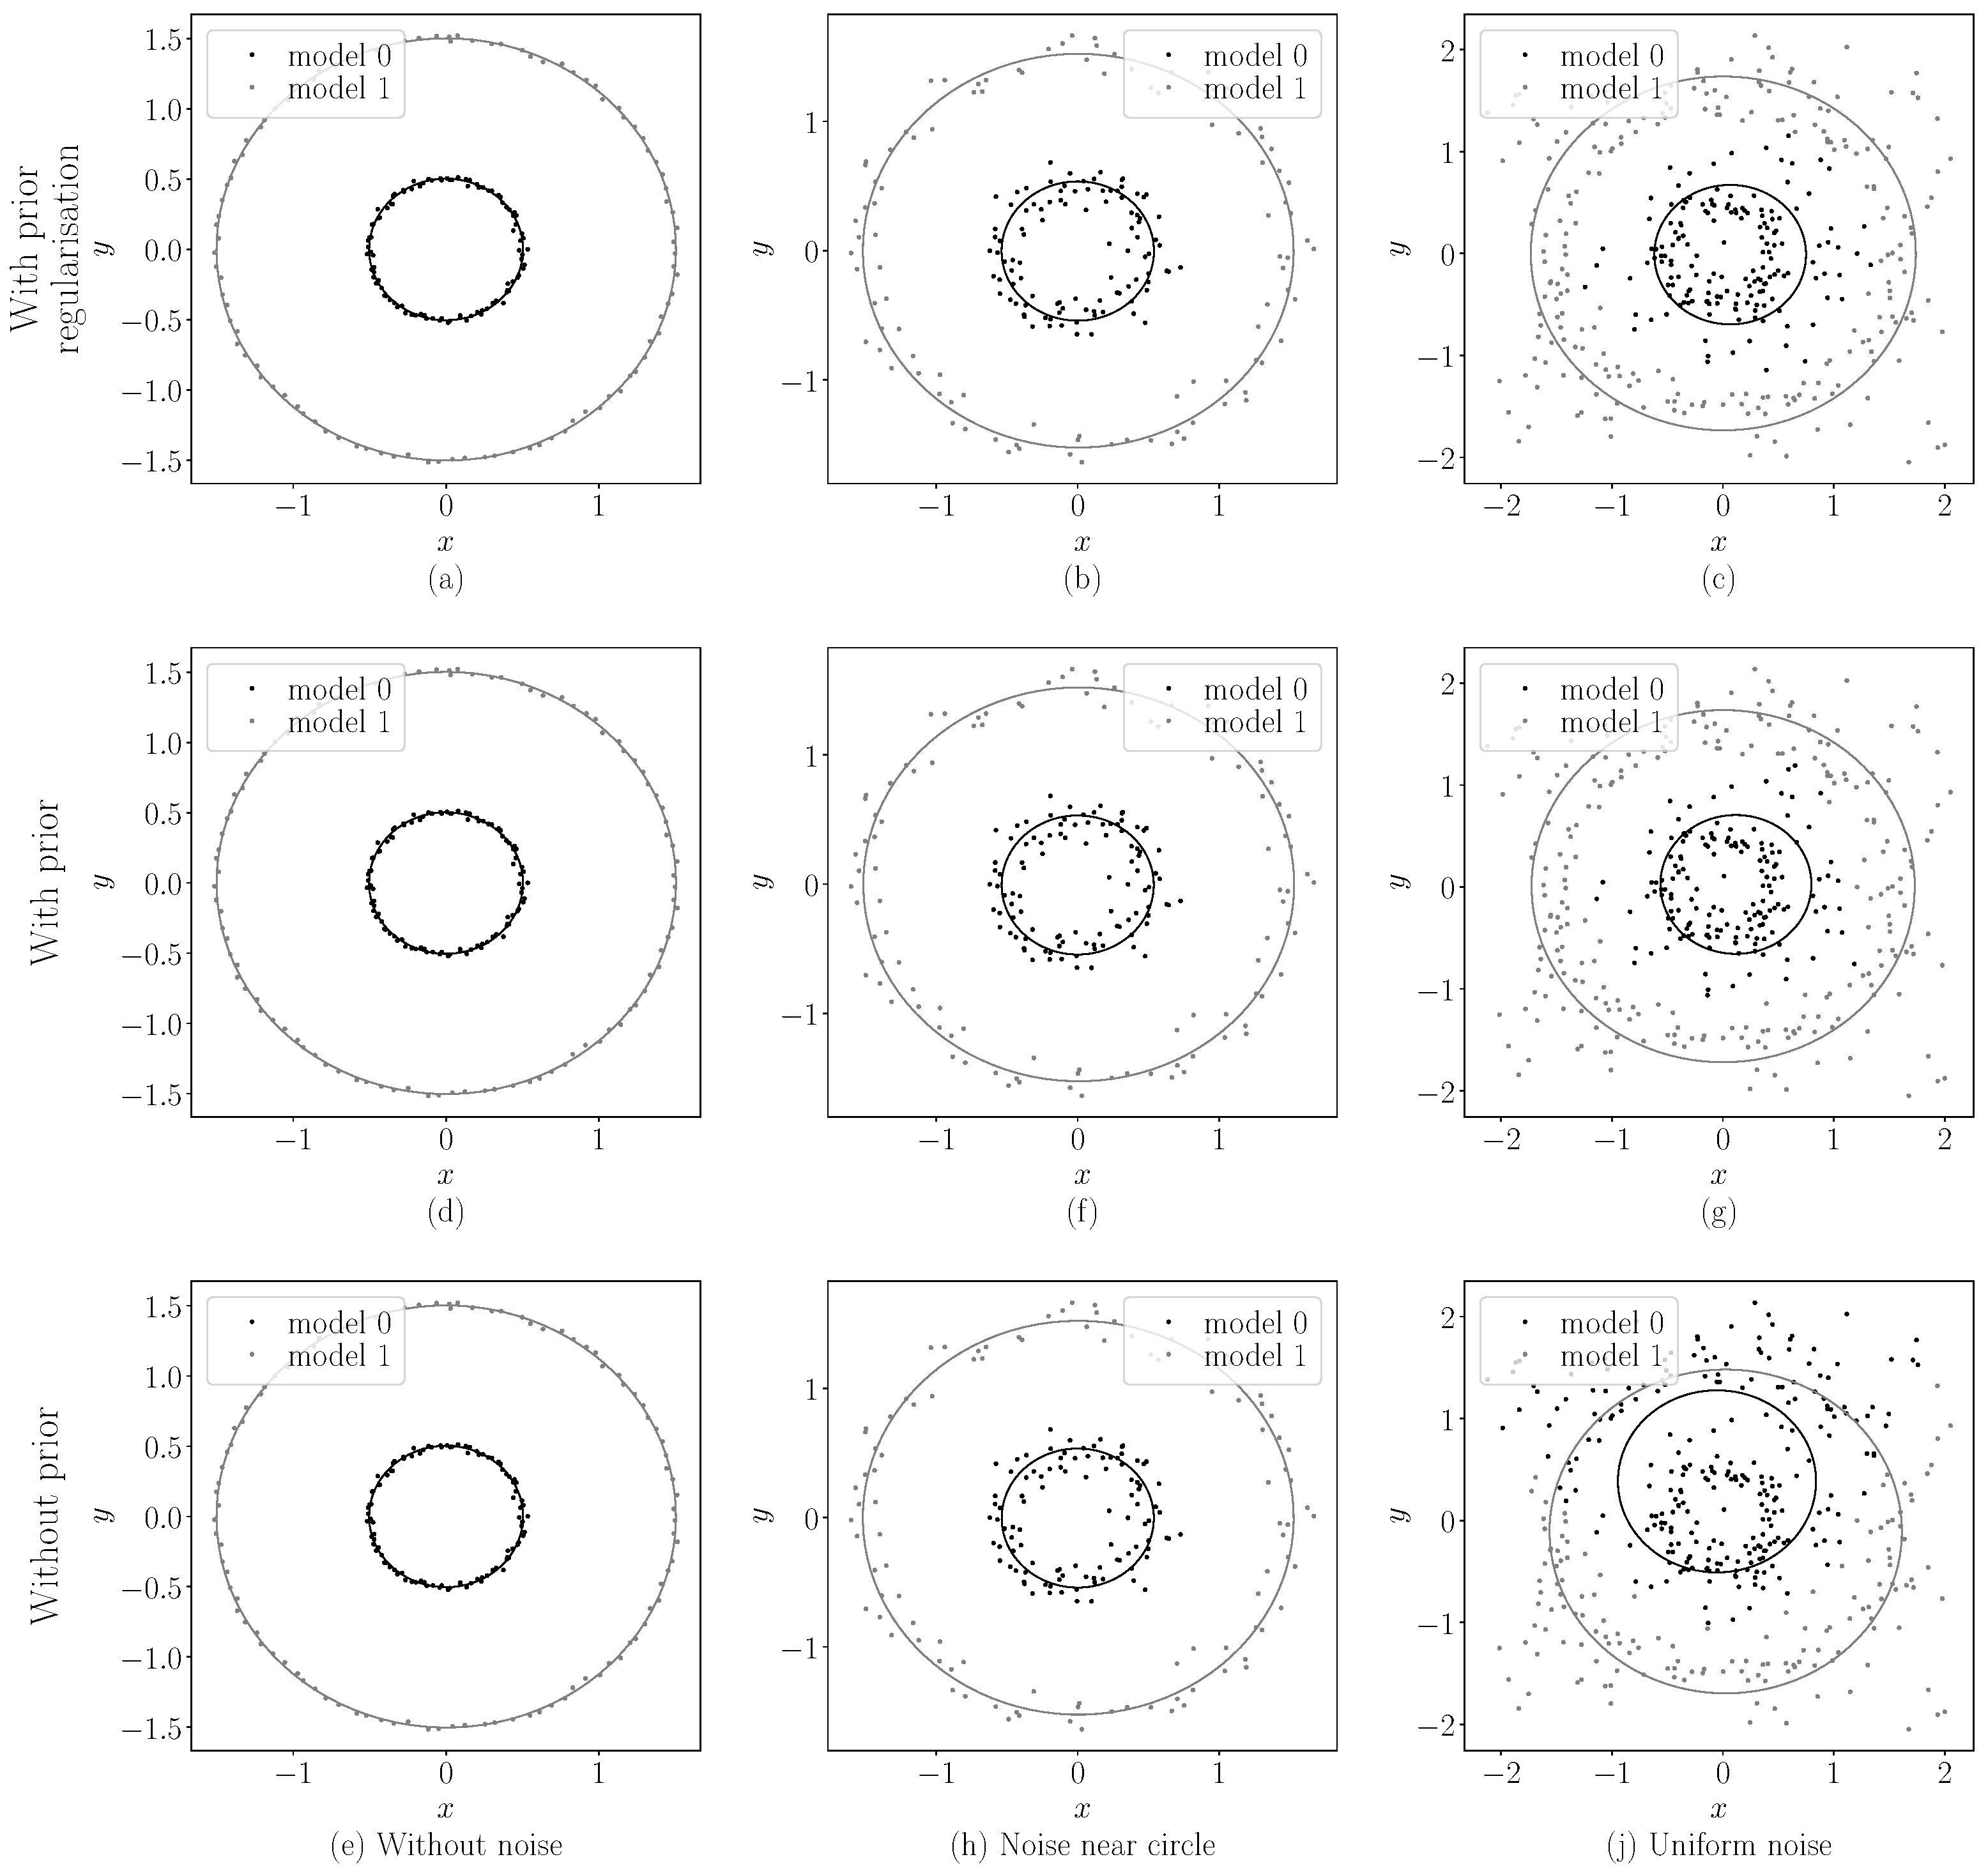
\includegraphics[width=1\textwidth]{results/priorexpert/experiment_synthetic}
\caption{Мультимодель в зависимости от разных априорных предположений и в зависимости от разного уровня шума: (a)--(с) модель с регуляризаций априорных распределений; (d)--(g) модель с заданными априорными распределениями на параметрах локальных моделей; (e)--(j) модель без заданных априорных предположений}
\label{ch4-experiment:1}
\end{figure}
В вычислительном эксперименте сравнивается качество мультимоделей~$\textbf{f}_1, \textbf{f}_2, \textbf{f}_3$ на синтетических данных.
Синтетические данные являются двумя концентрическими окружностями с разным уровнем шума.
Выборка Synthetic 1 является изображением без шума, выборка Synthetic 2 изображение с зачумлённым радиусом окружности, а выборка Synthetic 3 --- изображение с равномерным шумом.
На рис. \ref{ch4-experiment:1} показаны результаты для мельтимоделей~$\textbf{f}_1, \textbf{f}_2, \textbf{f}_3$.
Все модели оптимизировались при помощи 50 итераций EM-алгоритма.
Мультимодели~$\textbf{f}_2, \textbf{f}_3$ аппроксимируют окружности лучше чем мультимодель~$\textbf{f}_1$. В табл. \ref{tb:ce:1} показано качество аппрроксимации \eqref{ch4-eq:ce:ex:0:1} для всех мультимоделей.

\begin{table}[h!t]
\begin{center}
\caption{Качество аппроксимации мультимодели в зависимости от априорных распределений}
\label{tb:ce:1}
\begin{tabular}{|c|c|c|c|}
\hline
	Выборка &~$\mathcal{S}_{\textbf{f}_1}$ &~$\mathcal{S}_{\textbf{f}_2}~$&~$\mathcal{S}_{\textbf{f}_3}~$\\
	\hline
	\multicolumn{1}{|l|}{Synthetic 1}
	&~$10^{-5}$&~$10^{-5}$&~$10^{-5}$\\
	\hline
	\multicolumn{1}{|l|}{Synthetic 2}
	&~$0.6$&~$10^{-3}$&~$10^{-3}$\\
	\hline
	\multicolumn{1}{|l|}{Synthetic 3}
	&~$0.6$&~$10^{-3}$&~$10^{-3}$\\
\hline
\end{tabular}
\end{center}
\end{table}

\paragraph{Анализ сходимости на синтетической выборке.}
\begin{figure}[h!t]\center
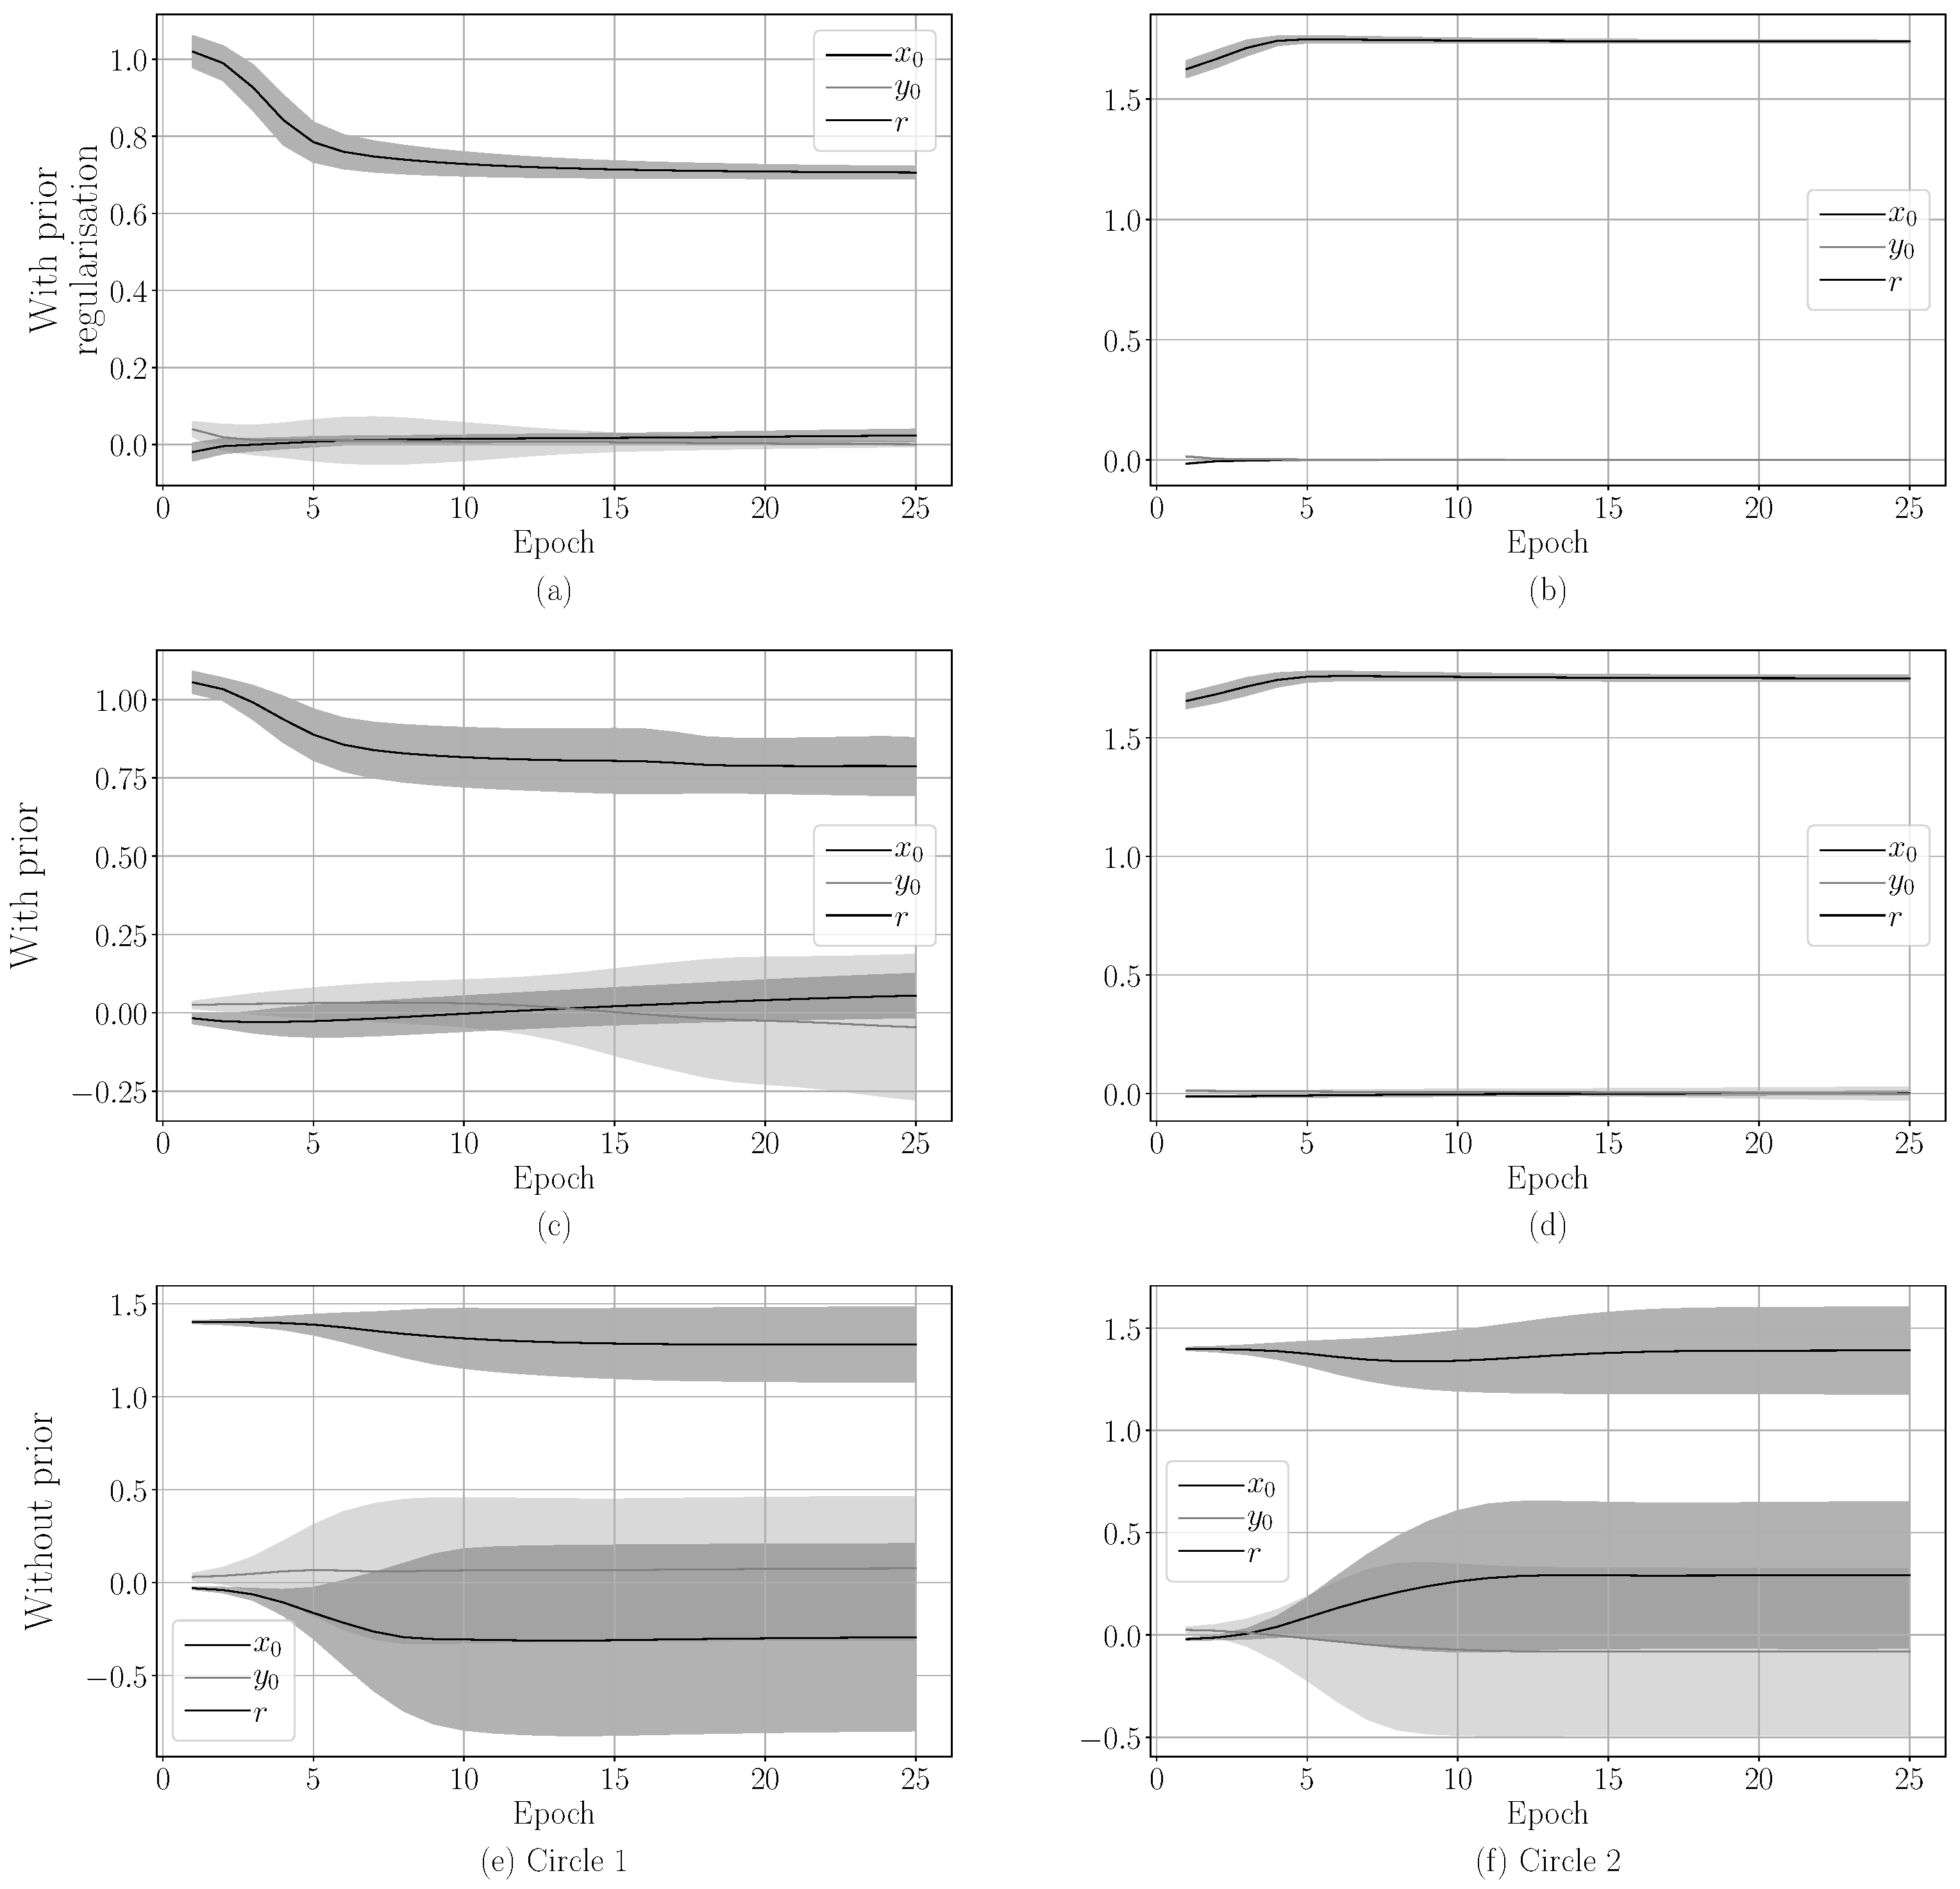
\includegraphics[width=1\textwidth]{results/priorexpert/experiment_synthetic_param_progress}
\caption{График зависимости центра и радиуса окружностей от номера итерации: (a)--(b) модель с регуляризацией априорных распределений; (c)--(d) модель с заданными априорными распределениями на параметры моделей; (e)--(f) модель без задания априорных распределений}
\label{ch4-experiment:st:2:1}
\end{figure}

\begin{figure}[h!t]\center
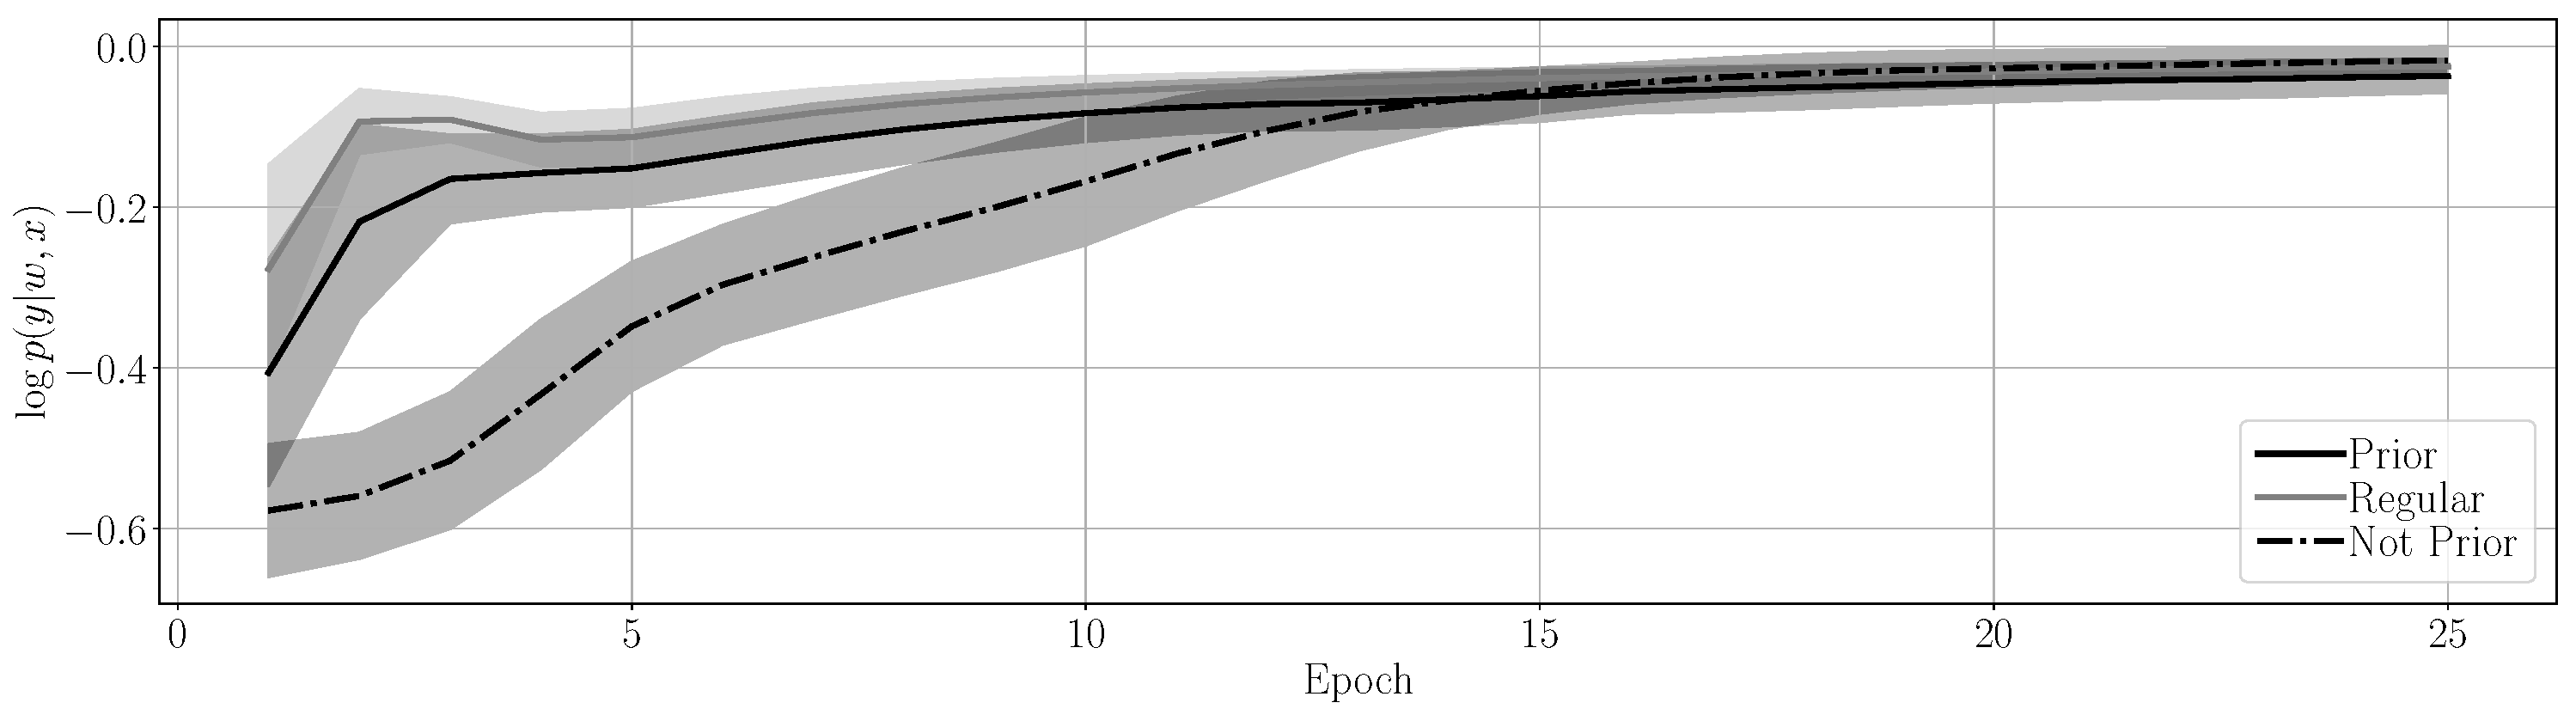
\includegraphics[width=1\textwidth]{results/priorexpert/experiment_synt_likelihood_progress}
\caption{График зависимости логарифма правдоподобия \eqref{ch4-eq:st:new:1} от номера итерации}
\label{ch4-experiment:st:2:2}
\end{figure}

\begin{figure}[h!t]\center
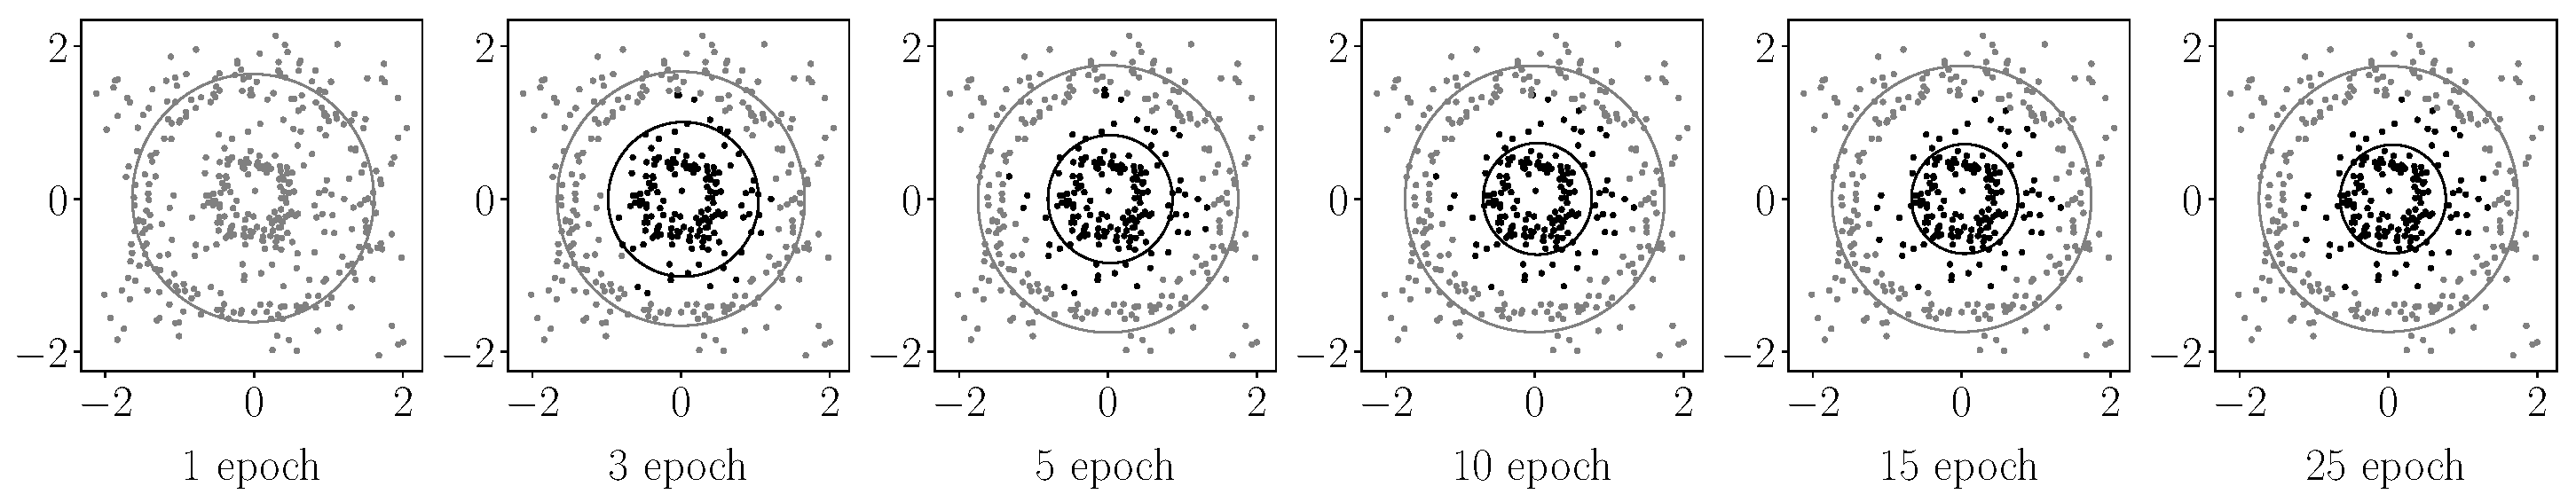
\includegraphics[width=1\textwidth]{results/priorexpert/experiment_synt_regular_progress}
\caption{Визуализации процесса сходимости мультимодели с использованием априорной регуляриции}
\label{ch4-experiment:st:2:3}
\end{figure}

\begin{figure}[h!t]\center
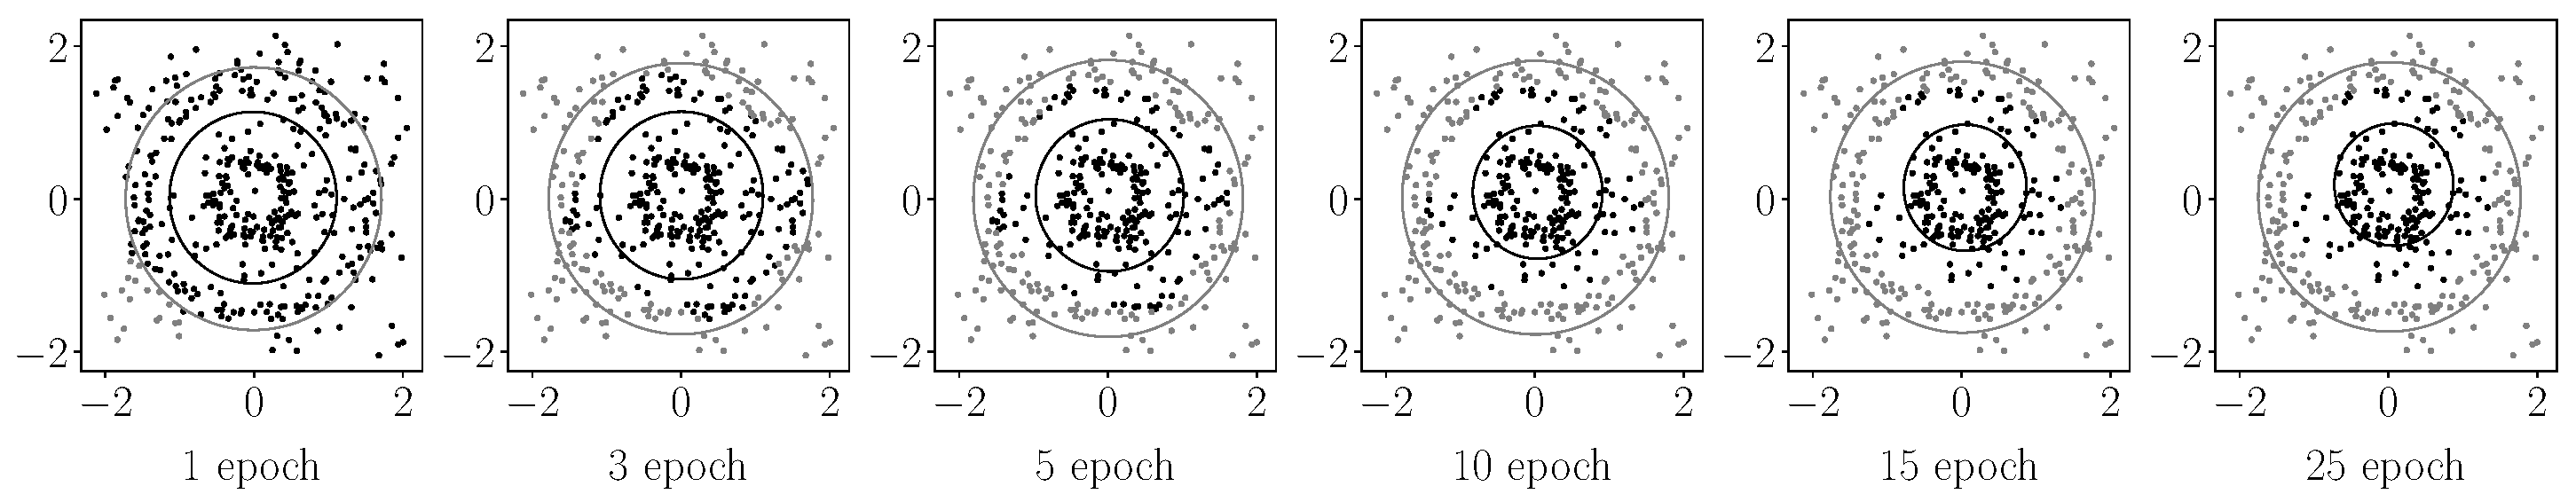
\includegraphics[width=1\textwidth]{results/priorexpert/experiment_synt_prior_progress}
\caption{Визуализации процесса сходимости мультимодели с использованием априорного распределением}
\label{ch4-experiment:st:2:4}
\end{figure}

\begin{figure}[h!t]\center
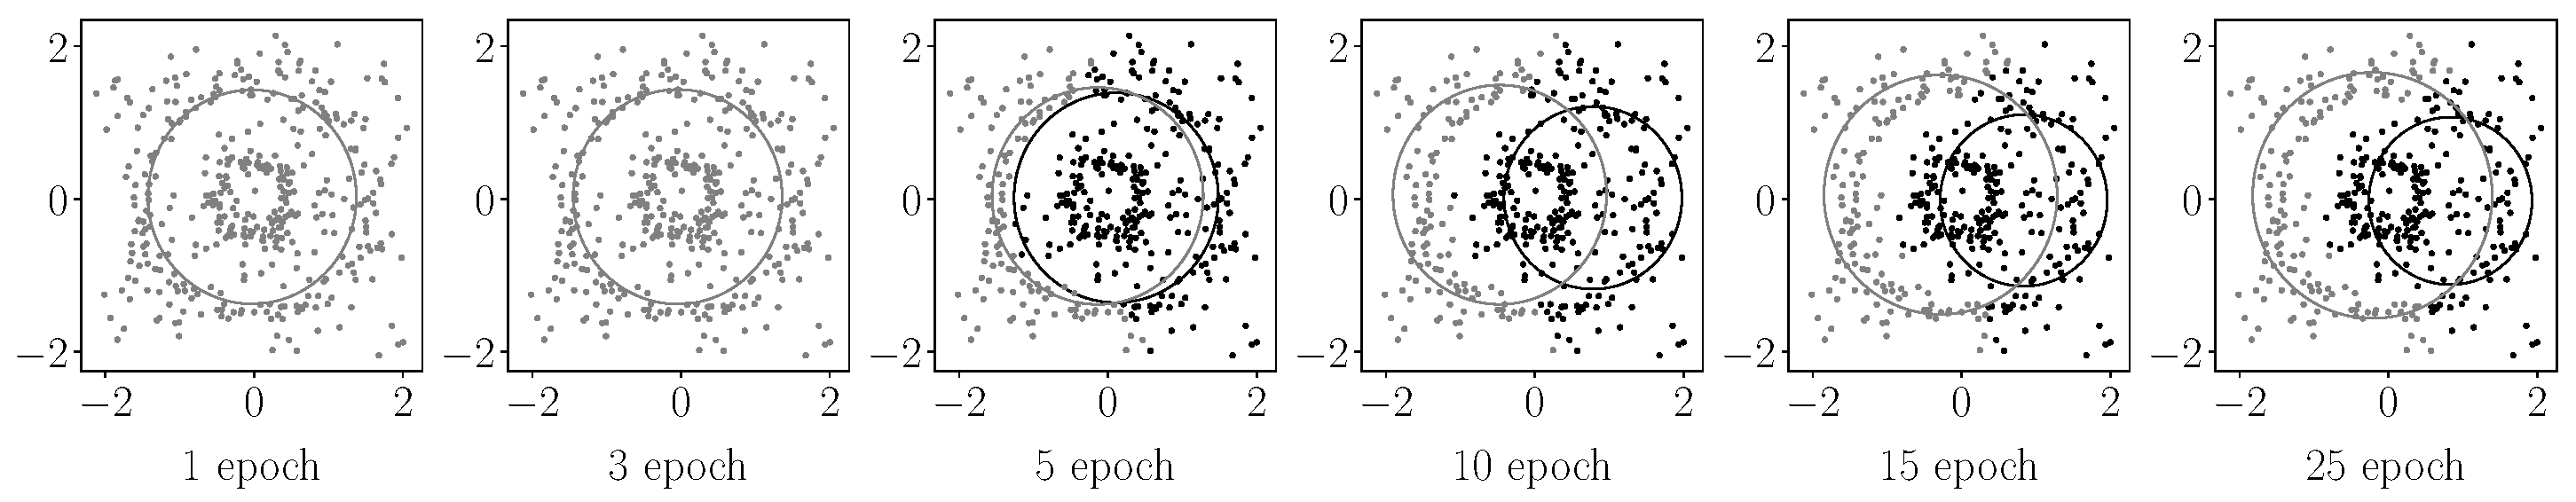
\includegraphics[width=1\textwidth]{results/priorexpert/experiment_synt_not_prior_progress}
\caption{Визуализации процесса сходимости мультимодели без использования априорного распределения}
\label{ch4-experiment:st:2:5}
\end{figure}
Данная часть эксперимента анализирует качество сходимости ЕМ-алгоритма для разных мультимоделей~$\textbf{f}_1, \textbf{f}_2, \textbf{f}_3$.
Анализ всех мультимоделей проводиться на выборке Synthetic 3.

На рис. \ref{ch4-experiment:st:2:1} показана зависимость предсказано центра и радуса в зависимости от номера итерации ЕМ-алгоритма.
Мультимодель~$\textbf{f}_2,$ использующая априорное распределение, аппроксимирует окружность лучше мультимодели~$\textbf{f}_1,$ которая не использует никакого априорного распределения.
Мультимодель~$\textbf{f}_3,$ использующая регуляризатор априорных распределений, является более стабильной, чем мультимодель~$\textbf{f}_2$.

На рис. \ref{ch4-experiment:st:2:2} показана зависимость логарифма правдоподобия \eqref{ch4-eq:st:new:1} от номера итерации EM-алгоритма.
Логарифм правдоподобия мультимодели~$\textbf{f}_2, \textbf{f}_3$ растет быстрее чем логарифм правдоподобия мультимодели~$\textbf{f}_1$.  После~$20$-й итерации все мультимодели имеют одинаковое правдоподобие.

На рис. \ref{ch4-experiment:st:2:3}-\ref{ch4-experiment:st:2:5} показан процесс сходимости для разных мультимоделей~$\textbf{f}_1, \textbf{f}_2, \textbf{f}_3$.
На рис. \ref{ch4-experiment:st:2:5} показана мультимодель~$\textbf{f}_1$, которая аппроксимирует окружности не верно.
На рис. \ref{ch4-experiment:st:2:3}-\ref{ch4-experiment:st:2:4} показаны мультимодели~$\textbf{f}_2, \textbf{f}_3$, которые аппроксимируют окружности верно.

Вычислительный эксперимент показывает, что мультимодели~$\textbf{f}_2, \textbf{f}_3,$ использующие априорные распределения на параметры экспертов, аппроксимируют окружности лучше чем мультимодель~$\textbf{f}_1,$ которая работает без априорных распределений.


\paragraph{Анализ мультимоделей в зависимости от уровня шума.} 
\begin{figure}[h!t]\center
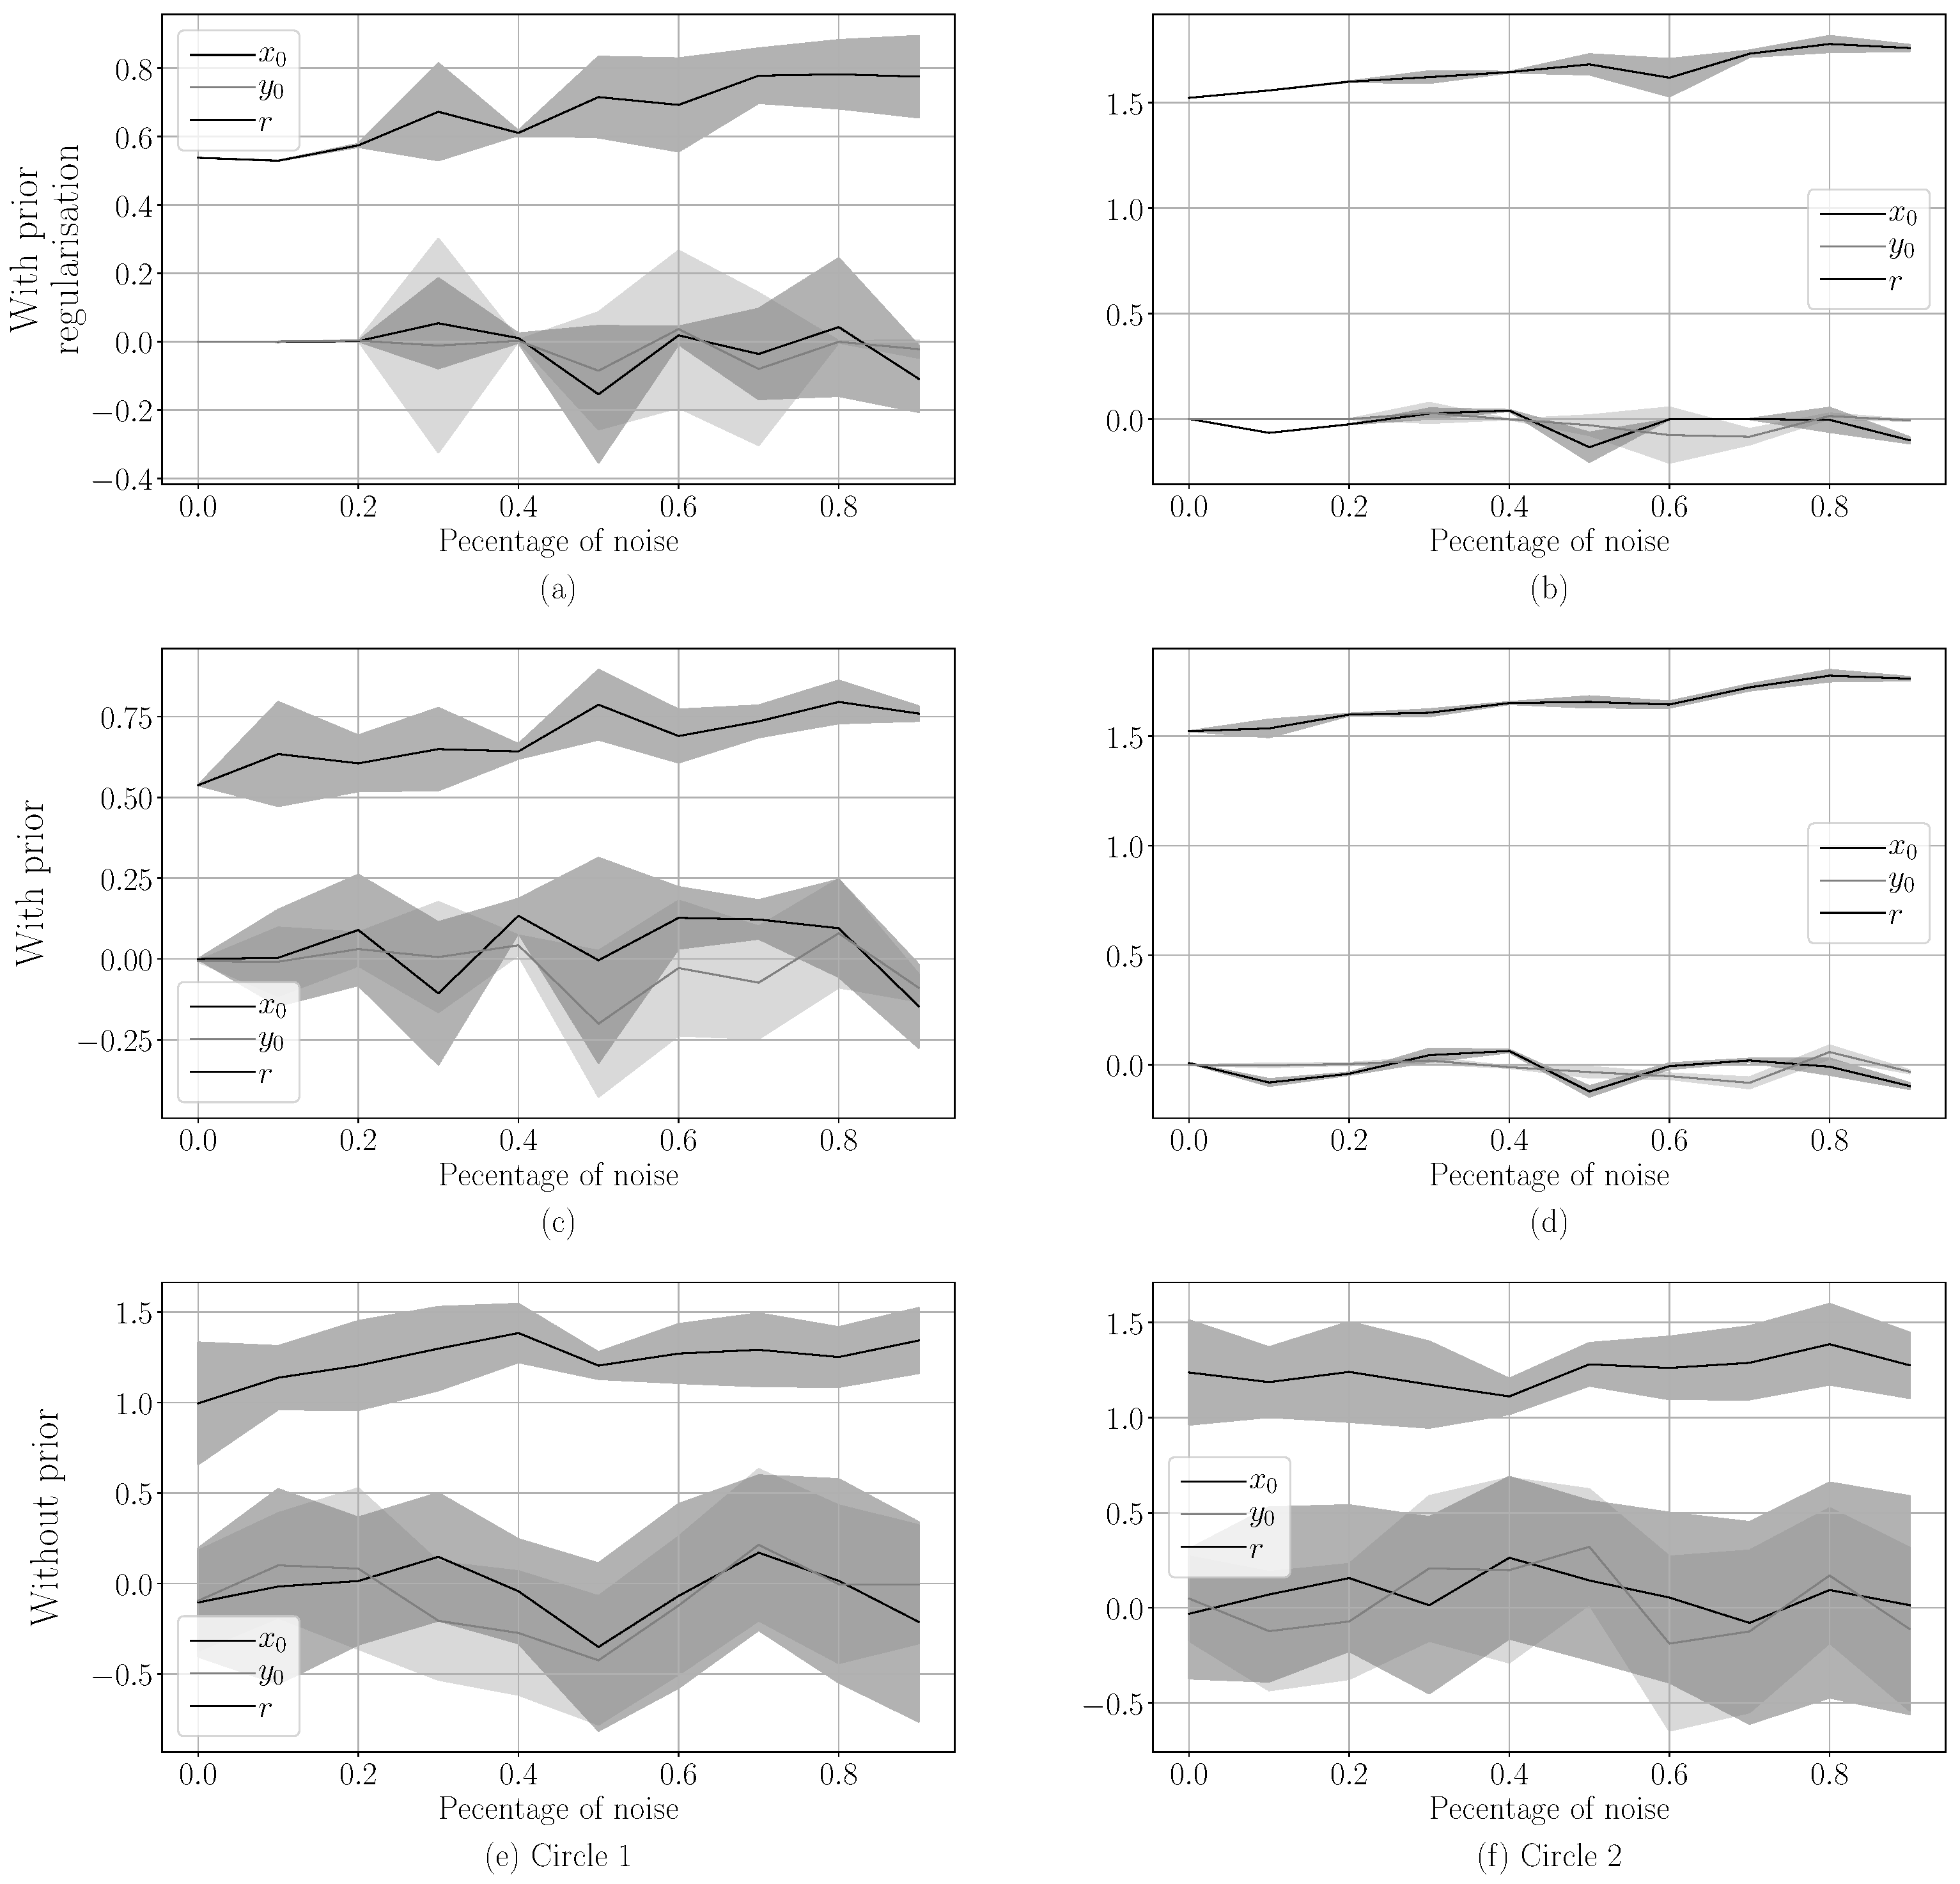
\includegraphics[width=1\textwidth]{results/priorexpert/experiment_synthetic_param_progress_noise}
\caption{График зависимости центра и радиуса окружностей от номера итерации: (a)--(b) модель с регуляризацией априорных распределений; (c)--(d) модель с заданными априорными распределениями на параметры моделей; (e)--(f) модель без задания априорных распределений}
\label{ch4-experiment:st:3:1}
\end{figure}

\begin{figure}[h!t]\center
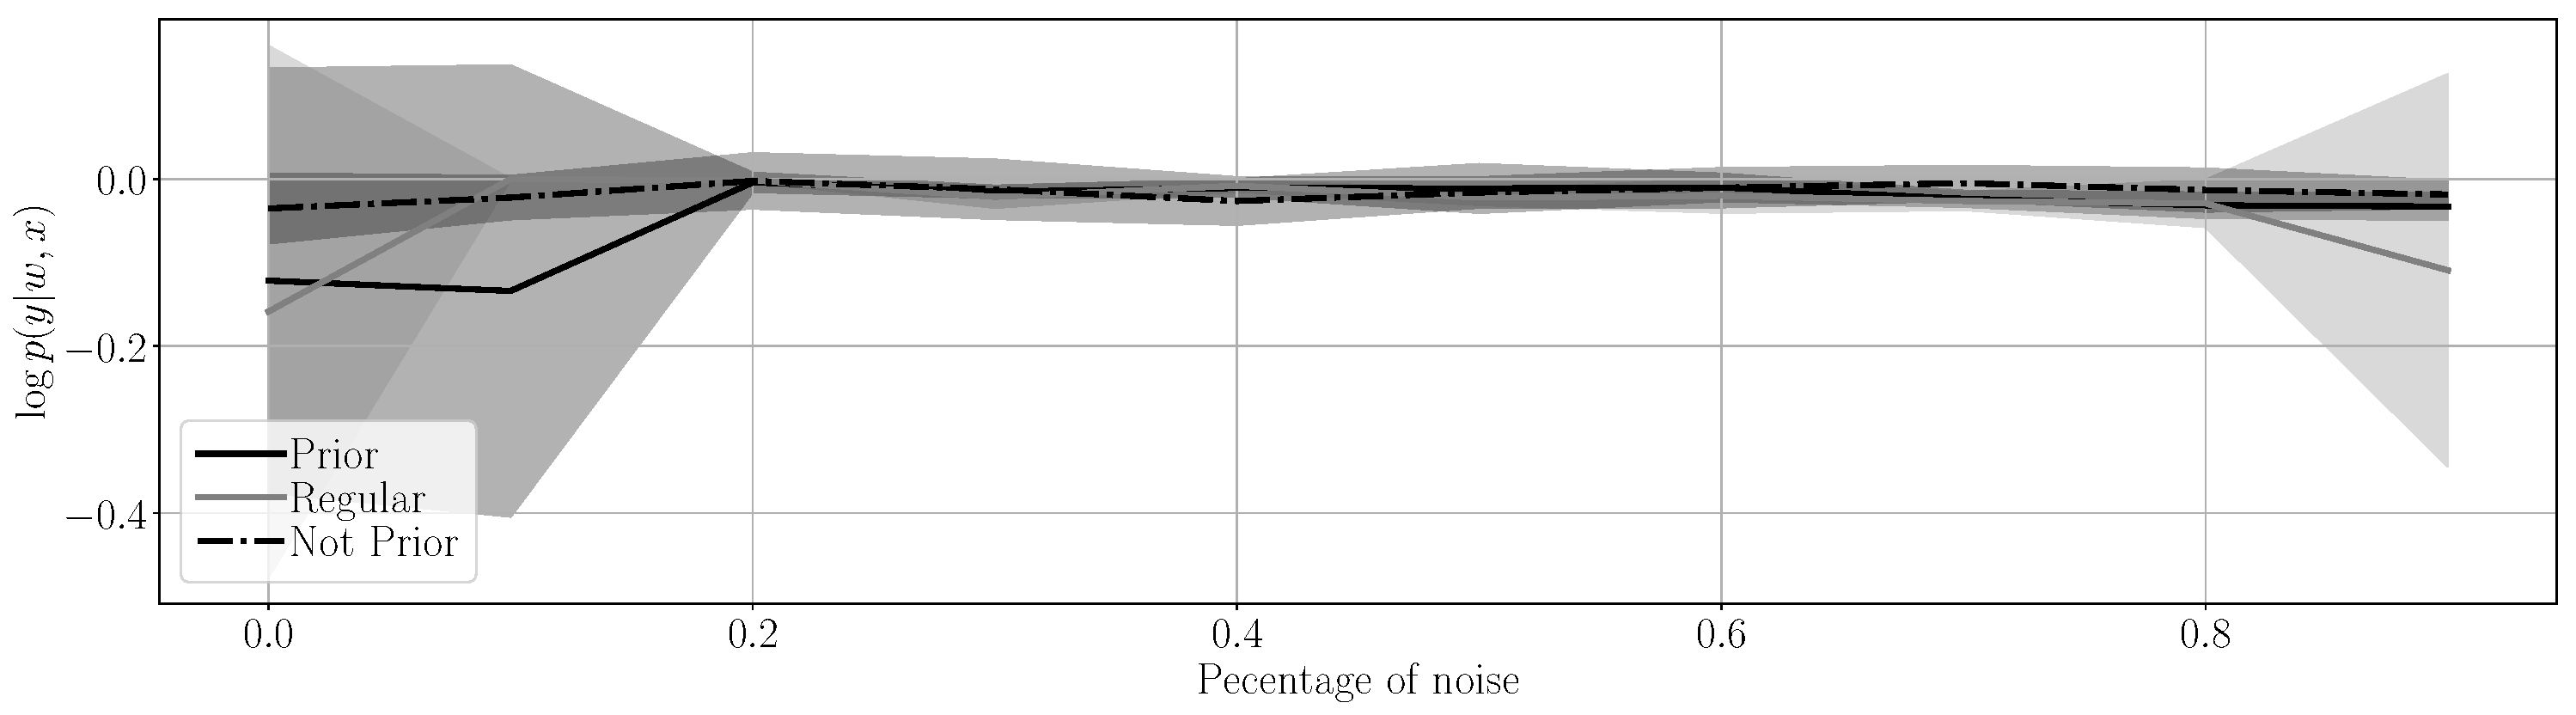
\includegraphics[width=1\textwidth]{results/priorexpert/experiment_synt_likelihood_progress_noise}
\caption{График зависимости логарифма правдоподобия \eqref{ch4-eq:st:new:1} от уровня шума
}
\label{ch4-experiment:st:3:2}
\end{figure}

Данная часть эксперимента анализирует зависимость разных мультимоделей~$\textbf{f}_1, \textbf{f}_2, \textbf{f}_3$ от уровня шума. 
Анализ всех мультимоделей проводиться на выборке Synthetic 1, с добавлением разного уровня шума.
Минимальный уровень шума равен~$0$, когда числа шумовых точек равно~$0$. Максимальный уровень шума равен~$1$, когда число шумовых точек равно числу точек на изображении.
На рис. \ref{ch4-experiment:st:3:1} показан график зависимости центра окружности и ее радиус в зависимости от уровня шума. Из графика видно, что радиус окружности увеличивается при увеличении уровня шума. 
Мультимодели~$\textbf{f}_2, \textbf{f}_3$ аппроксимируют центр окружности верно, но мультимодель~$\textbf{f}_3$ более устойчива к шуму .
На рис. \ref{ch4-experiment:st:3:2} показана зависимость логарифма правдоподобия \eqref{ch4-eq:st:new:1} от уровня шума. 
Из графика видно, что логарифм правдоподобия \eqref{ch4-eq:st:new:1} эквивалентный для всех мультимоделей, но на рис. \ref{ch4-experiment:st:3:1} видно, что качество аппроксимации \eqref{ch4-eq:ce:ex:0:1} зависит от мультимодели.
Данная часть вычислительного эксперимента показывает, что мультимодель~$\textbf{f}_3$ с регуляризацией априорного распределения является более устойчива к шуму, чем остальные.

\paragraph{Реальные данные.}
\begin{figure}[h!t]\center
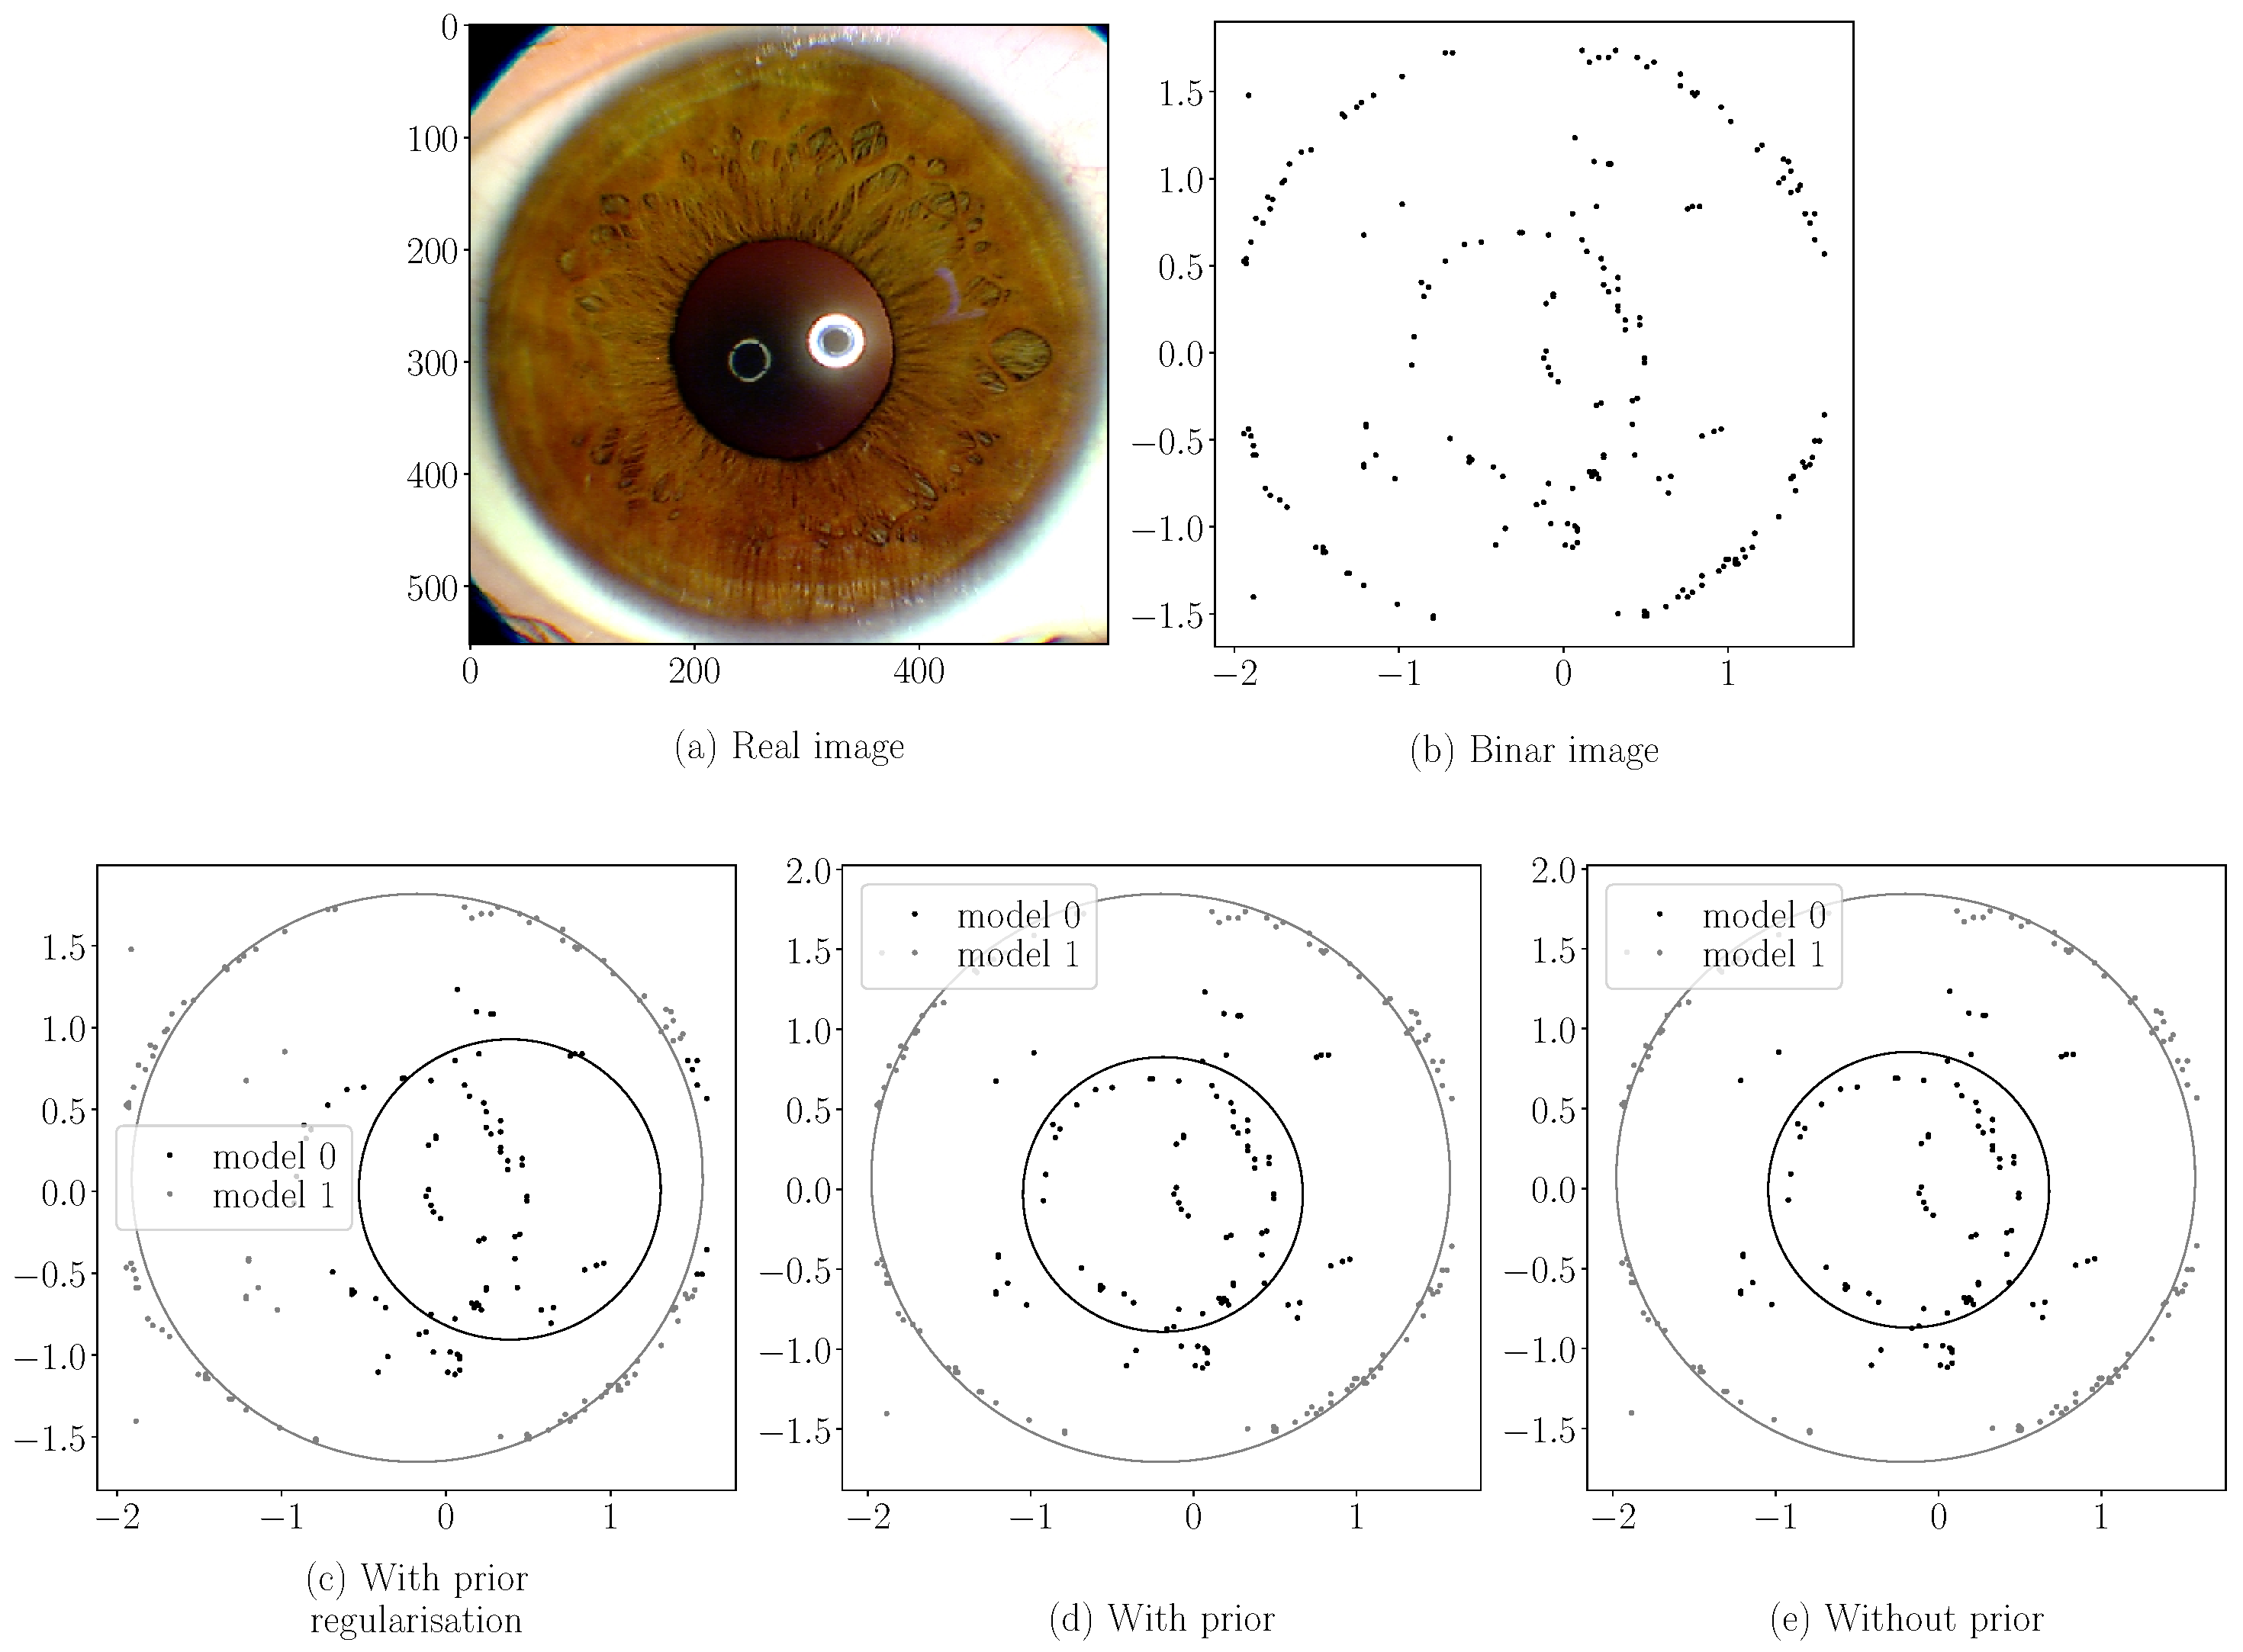
\includegraphics[width=0.9\textwidth]{results/priorexpert/experiment_real_compare}
\caption{Мультимодель в зависимости от разных априорных предположений на реальном изображении: (a) исходное изображение; (b) бинаризованое изображение; (c) мультимодель без априорных предположений; (d) мультимодель с априорными распределениями на параметрах локальных моделей; (e) мультимодель с регуляризаций на априорных распределениях параметров локальных моделей}
\label{ch4-experiment:2}
\end{figure}

Данная часть эксперимента анализирует разные мультимодели~$\textbf{f}_1, \textbf{f}_2, \textbf{f}_3$ на реальной выборке.
На рис. \ref{ch4-experiment:2} показан результат работы разных мультимоделей.
Мультимодель~$\textbf{f}_1$  не верно аппроксимирует меньшую окружность.
Мультимодели~$\textbf{f}_2, \textbf{f}_3$ аппроксимируют обе окружности верно.

\begin{figure}[h!t]\center
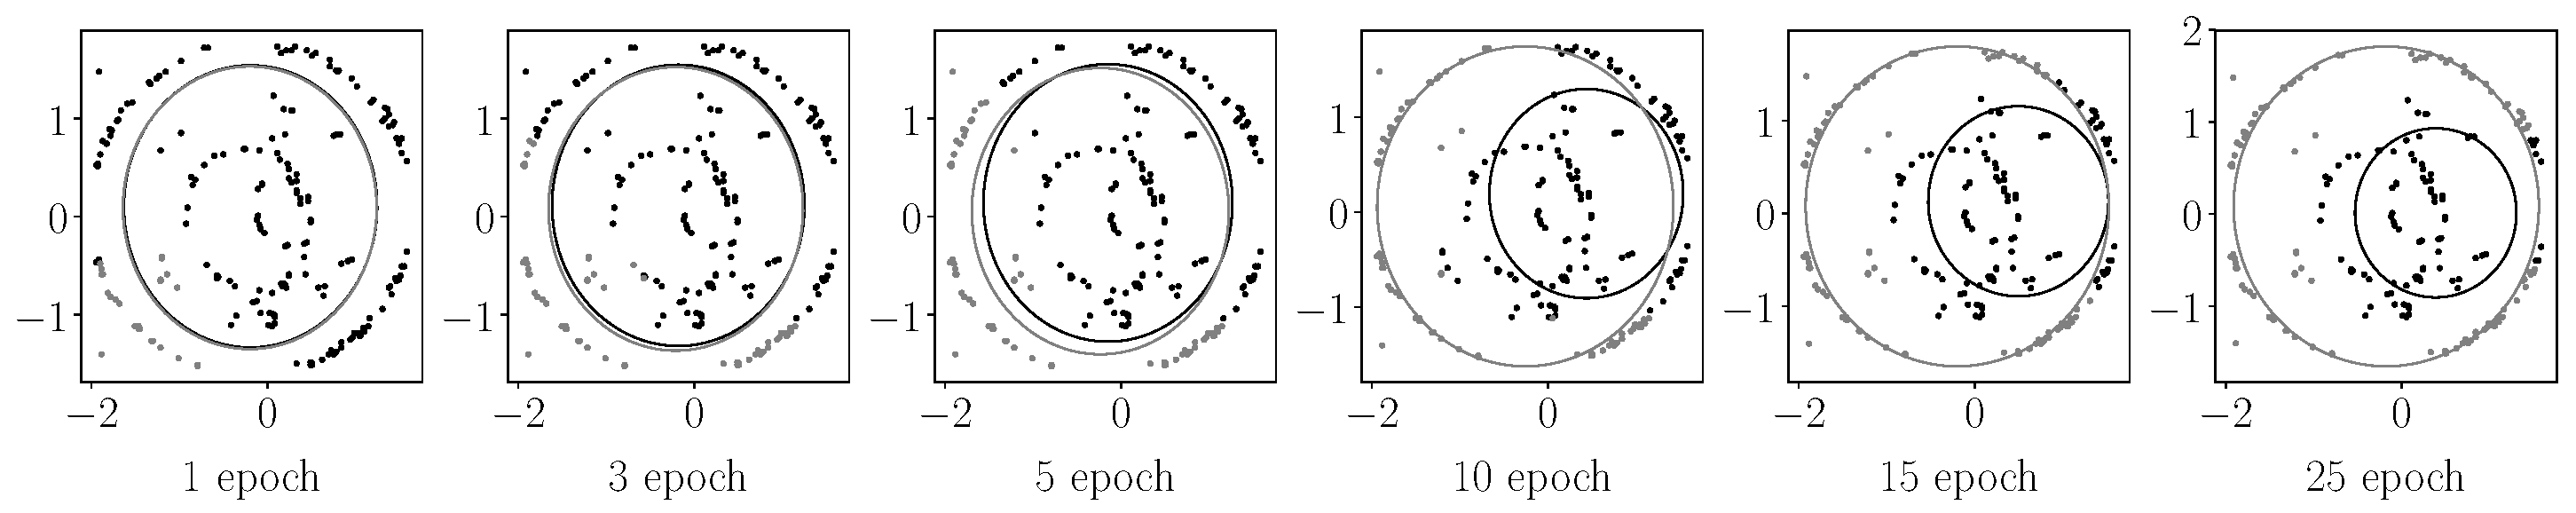
\includegraphics[width=1\textwidth]{results/priorexpert/experiment_real_not_prior}
\caption{Визуализации процесса сходимости мультимодели без использования априорного распределения}
\label{ch4-experiment:3}
\end{figure}

\begin{figure}[h!t]\center
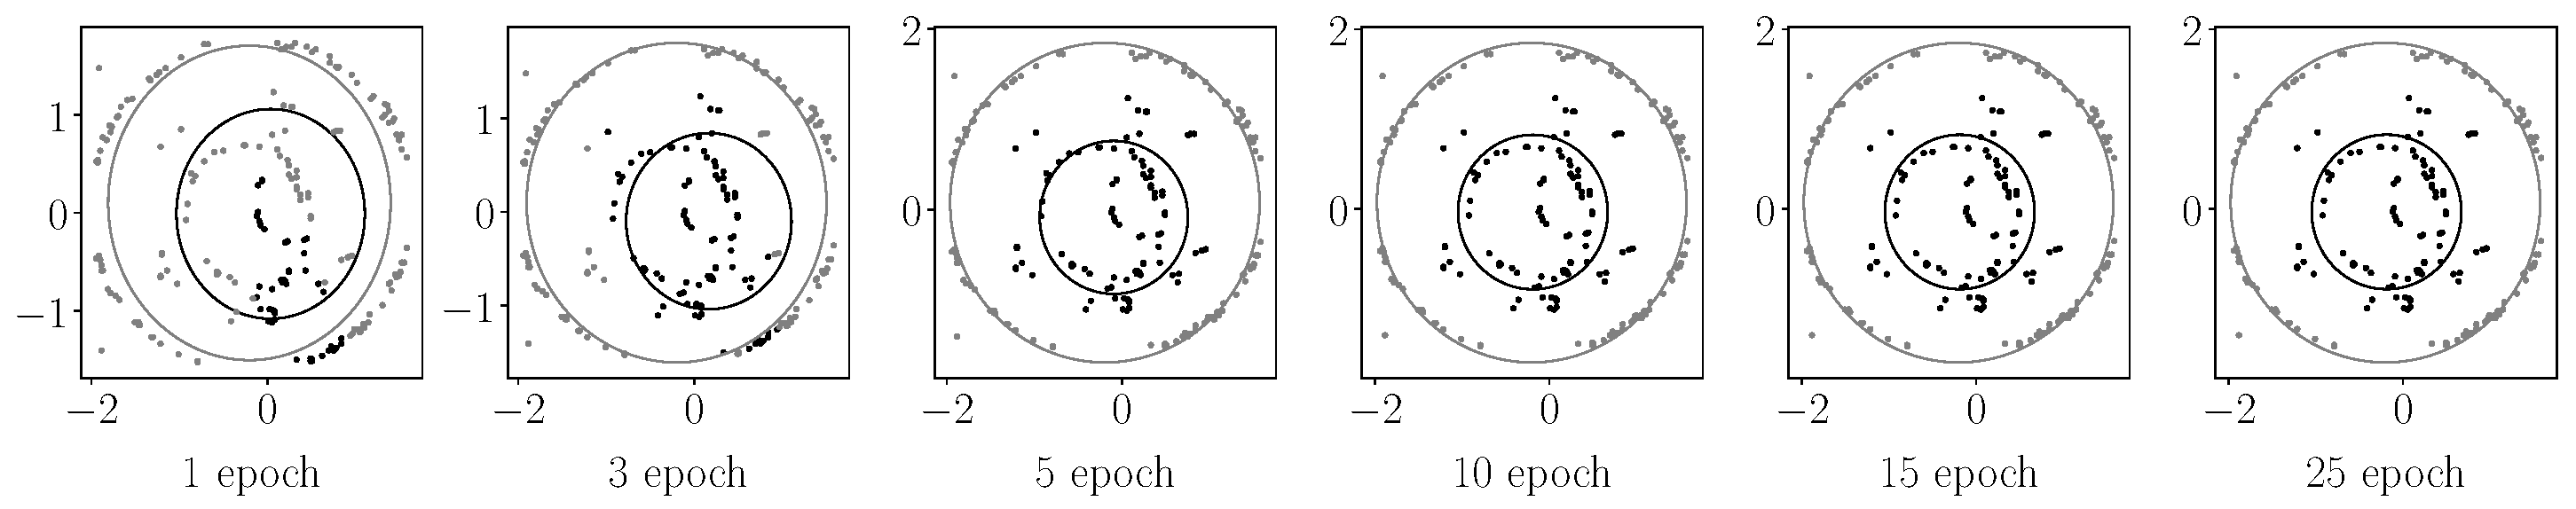
\includegraphics[width=1\textwidth]{results/priorexpert/experiment_real_prior}
\caption{Визуализации процесса сходимости мультимодели с использованием априорного распределением}
\label{ch4-experiment:4}
\end{figure}

\begin{figure}[h!t]\center
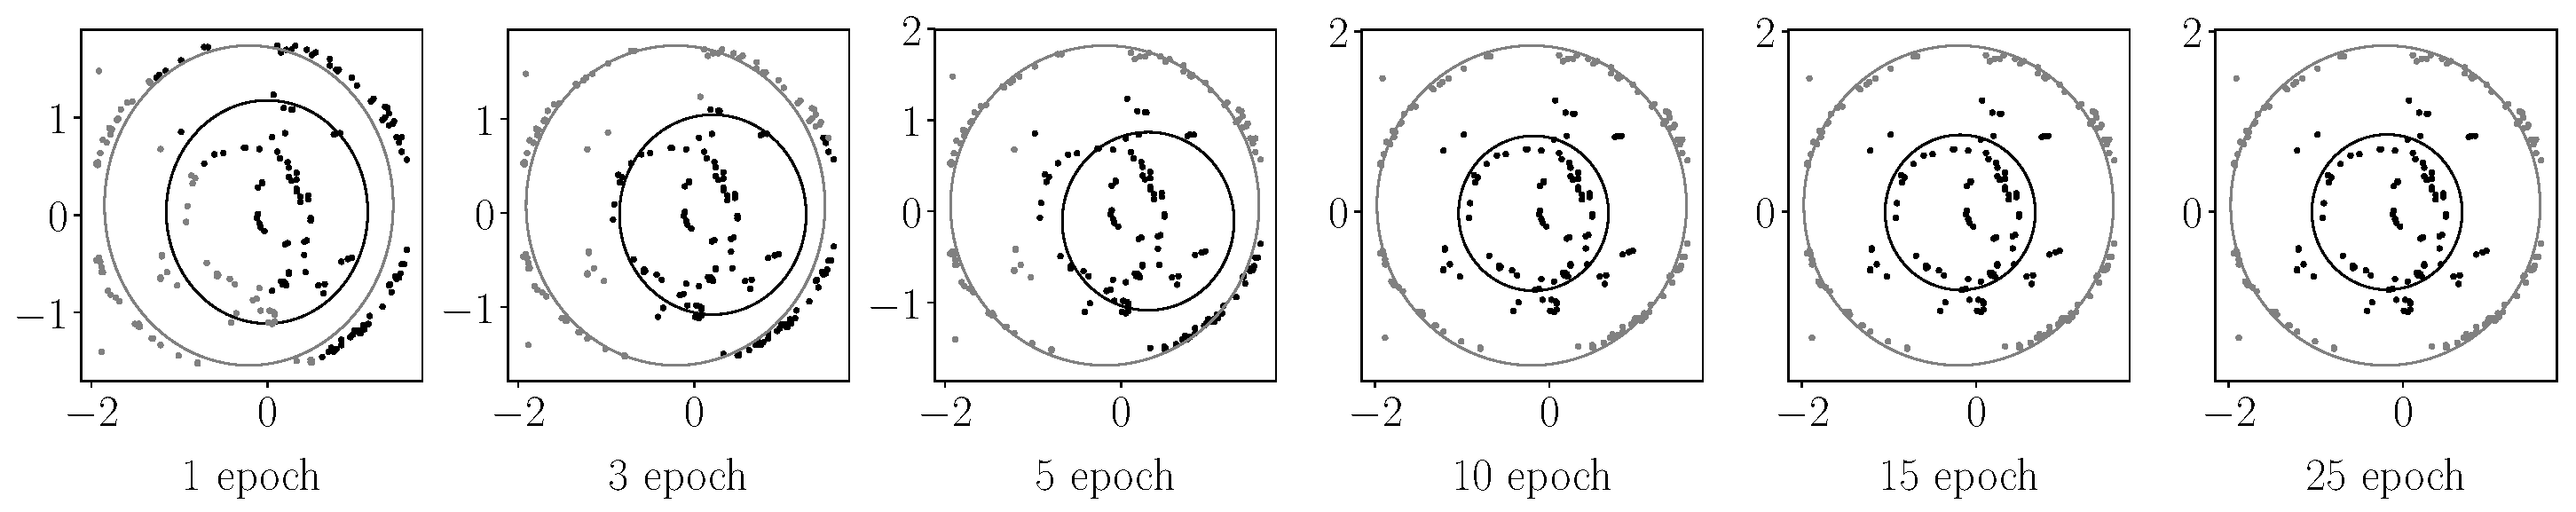
\includegraphics[width=1\textwidth]{results/priorexpert/experiment_real_regular}
\caption{Визуализации процесса сходимости мультимодели с использованием априорной регуляриции}
\label{ch4-experiment:5}
\end{figure}

На рис. \ref{ch4-experiment:3}-\ref{ch4-experiment:5} показан процесс аппроксимации для разных мультимоделей~$\textbf{f}_1, \textbf{f}_2, \textbf{f}_3$.

Данная часть эксперимента показывает, что мультимодели~$\textbf{f}_2, \textbf{f}_3$ аппроксимируют окружности на реальных изображениях лучше, чем мультимодель~$\textbf{f}_1$.

Проведен вычислительный эксперимент по анализу качества моделей кривых второго порядка на изображении. Эксперимент разделен на несколько частей. Первая часть - это эксперимент с несколькими окружностями на изображении. Во второй части анализируется сходимость метода в зависимости от уровня шума в данных и от указанной экспертной информации. В третьей части проводится эксперимент по аппроксимации радужной оболочки глаза.

\begin{figure}[h!]
\center
	\subfloat[]{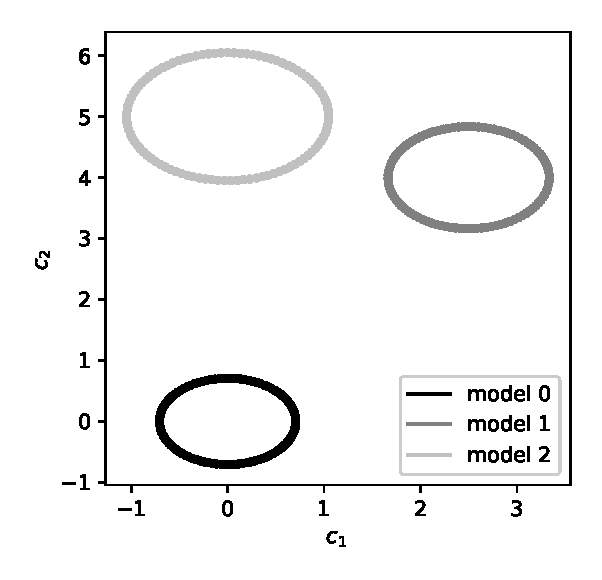
\includegraphics[height = 0.2\textheight]{results/priorexpertfig/900.eps}} 
	\subfloat[]{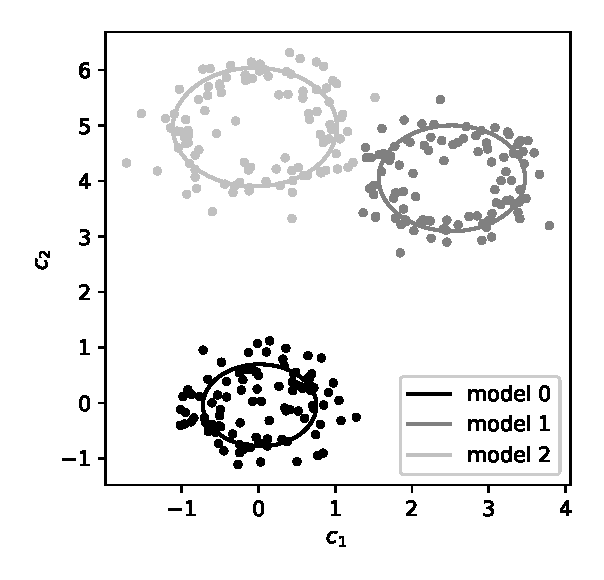
\includegraphics[height = 0.2\textheight]{results/priorexpertfig/901.eps}}
	\subfloat[]{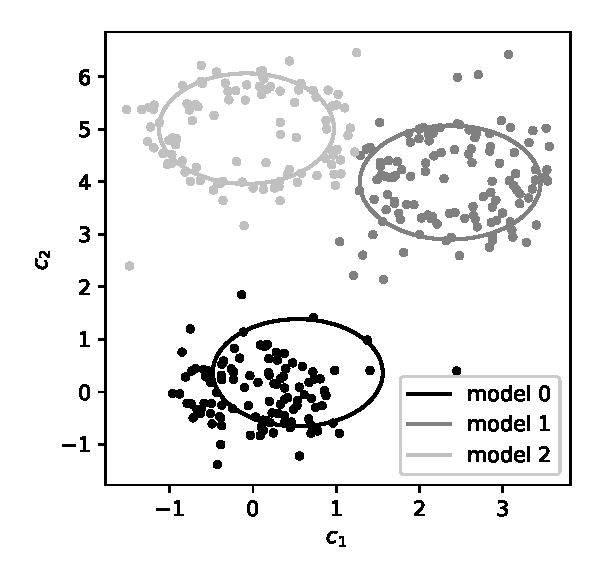
\includegraphics[height = 0.2\textheight]{results/priorexpertfig/902.eps}} 
\caption{Мультимодель в зависимости от различных предварительных предположений и уровня шума. Слева направо: окружности без шума; шум в радиусе круга; шум в радиусе круга, а также произвольные точки по всему изображению}
\label{ch4-ce:fig3}
\end{figure}

\begin{figure}[ht]
\center
	\subfloat[]{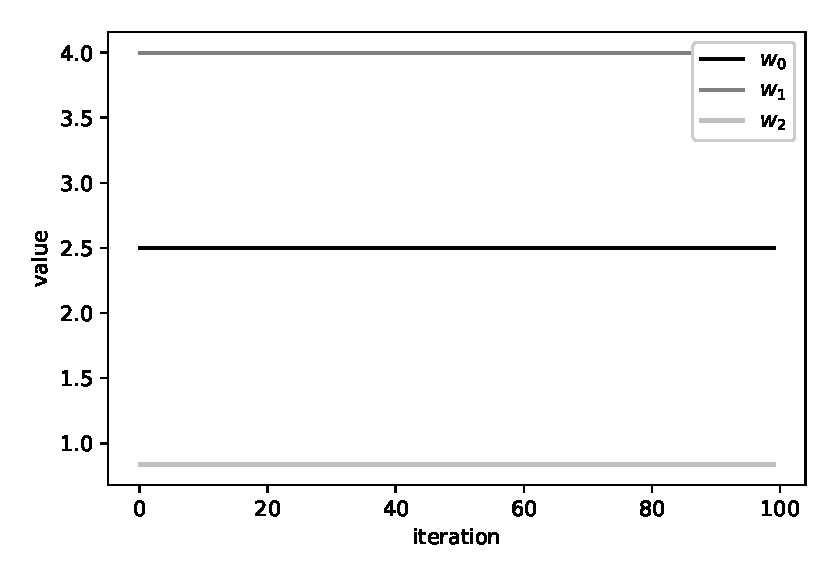
\includegraphics[height = 0.2\textheight]{results/priorexpertfig/900noise.eps}} 
	\subfloat[]{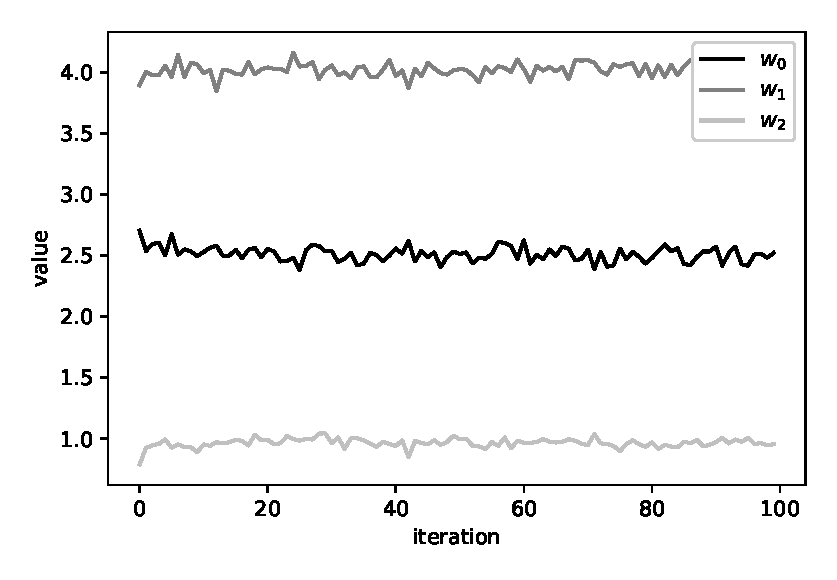
\includegraphics[height = 0.2\textheight]{results/priorexpertfig/901noise.eps}}\\
	\subfloat[]{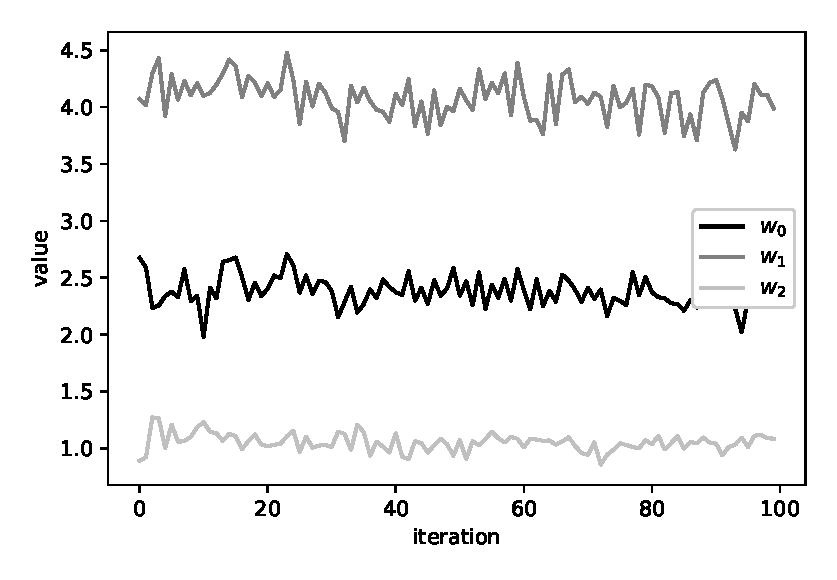
\includegraphics[height = 0.2\textheight]{results/priorexpertfig/902noise.eps}} 

\caption{Зависимость параметров~$r$,~$x_0$ и~$y_0$ от номера итерации для различных априорных распределений. Слева направо: окружности без шума; шум в радиусе круга; шум в радиусе круга, а также произвольные точки по всему изображению}
\label{ch4-ce:fig4}
\end{figure}

В этой части эксперимента показан пример обучения мультимодели для аппроксимации нескольких фигур второго порядка одновременно. В качестве данных используется синтетическая выборка с тремя произвольными непересекающимися окружностями, а также добавления шума к этим окружностям. Шум добавлен к радиусу круга для каждой точки, а также случайные точки добавлены к выборке.

На рисунке \ref{ch4-ce:fig3} показан результат построения ансамбля локально аппроксимирующих моделей, которые аппроксимируют образец. Каждая локальная модель аппроксимирует одну окружность, а при добавлении еще большего шума качество аппроксимации падает.
На рисунке \ref{ch4-ce:fig4} показан график зависимости радиуса окружностей~$ r~$ и их центров~$(x_0, y_0)$ от номера итерации.

\begin{figure}[h!t]
\center
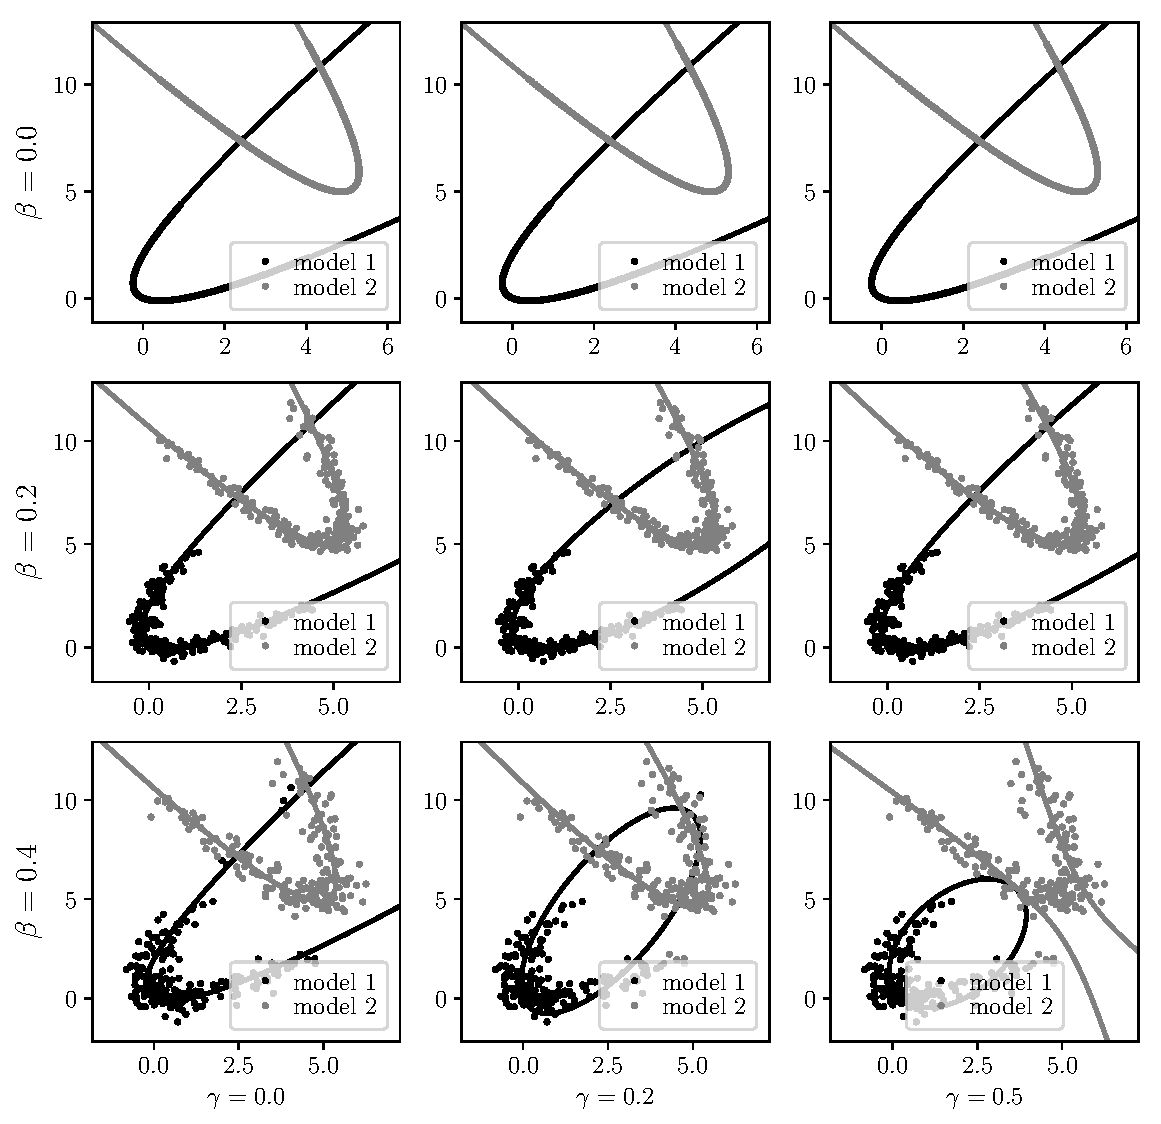
\includegraphics[width=0.8\textwidth]{results/priorexpertfig/beta_gamma}
\caption{Результат аппроксимации для данных с разными уровнями шума~$\beta$ и дисперсией априорного распределения~$\gamma$}
\label{ch4-ce:fig6}
\end{figure}

\begin{figure}[h!t]
\center
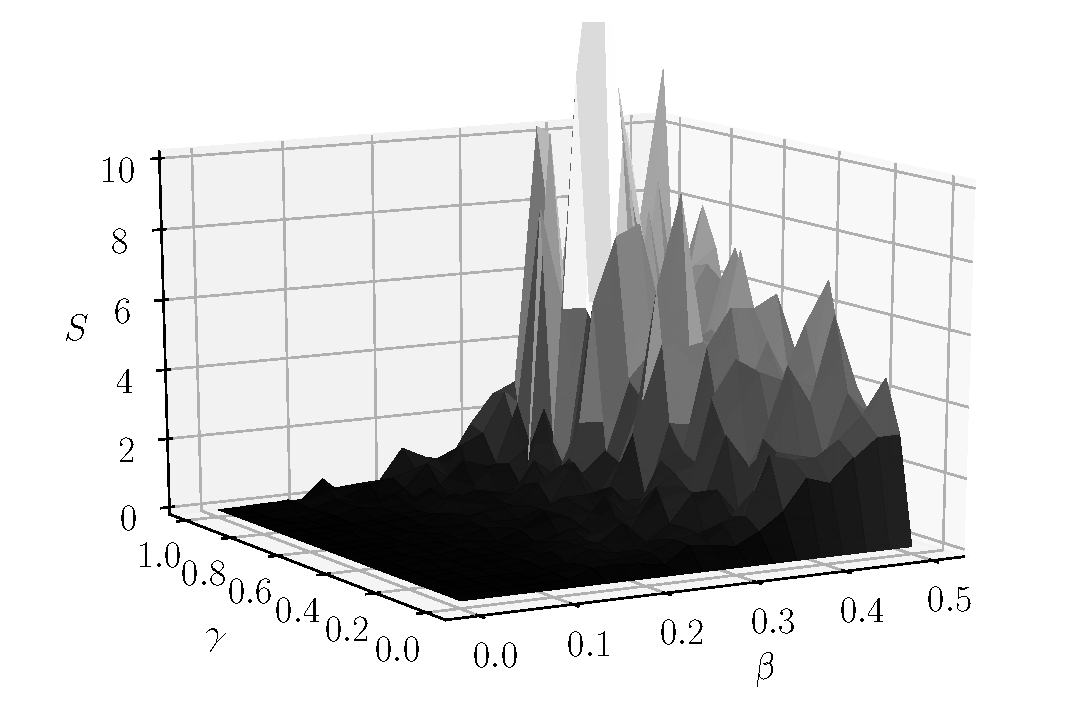
\includegraphics[width=0.5\textwidth]{results/priorexpertfig/3dplot}
\caption{Зависимость моделей от уровня шума~$\beta$ в данных, а также от дисперсии априорного распределения~$\gamma$}
\label{ch4-ce:fig5}
\end{figure}

В этой части эксперимента анализируется качество аппроксимации~$S$ в зависимости от уровня шума~$\beta$ в данных и по параметру априорных распределений~$\gamma$. Алгоритм генерации: сначала случайным образом выбираются два вектора параметров:~$\mathbf{w}^\text{true}_{1}$ и~$\mathbf{w}^\text{true}_{2}$ коэффициенты двух парабол. Векторы~$\mathbf{w}^\text{true}_{1}$ и~$\mathbf{w}^\text{true}_{2}$ используются для создания точек~$x_i$ и~$y_i$ с добавлением нормального шума~$\varepsilon\sim\mathcal{N}\bigr(0, \beta\bigr)~$. При обучении мультимодели, априорное распределение параметров считается~$\mathbf{w}_1\sim\mathcal{N}\bigr(\mathbf{w}^\text{true}_{1}, \gamma\mathbf{I}\bigr), \mathbf{w}_2\sim\mathcal{N}\bigr(\mathbf{w}^\text{true}_{2},\gamma\mathbf{I}\bigr)$.

Рассмотри критерий качества:
\[
S = ||\mathbf{w}^\text{pred}_{1} - \mathbf{w}^\text{true}_{1}||^{2}_{2} + ||\mathbf{w}^\text{pred}_{2} - \mathbf{w}^\text{true}_{2}||^{2}_{2},
\]
где~$\mathbf{w}^\text{pred}_{1}$ аппроксимация вектора параметров первой локальной модели, а~$\mathbf{w}^\text{pred}_{2}~$ аппроксимация вектора параметров второй локальной модели.

На рисунке \ref{ch4-ce:fig5} показана зависимость критерия качества~$S$ от уровня шума~$\beta$ и параметра априорного распределения~$\gamma$. График показывает, что при низком уровне шума~$\beta$ качество приближения не зависит от параметра~$\gamma$, а с увеличением шума~$\beta$ качество приближения~$S$ снижается.

На рисунке \ref{ch4-ce:fig5} показан пример того, как алгоритм работает с разными параметрами~$\beta$ и~$\gamma$. Видно, что в отсутствие шума~$\beta$ обе локальные модели аппроксимируют образец. С увеличением уровня шума качество аппроксимации снижается: при~$\beta = 0{,}2$ при увеличении~$\gamma$ первая локальная модель от параболы переходит в эллипс; при~$\beta = 0{,}4$ при увеличении~$\gamma$ первая локальная модель из параболы переходит в эллипс, а вторая модель из параболы переходит в гиперболу.

\begin{figure}[h!]
\center
	\subfloat[]{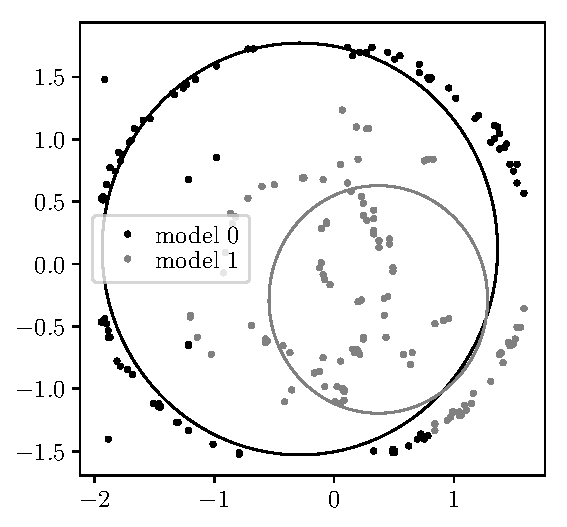
\includegraphics[height = 0.17\textheight]{results/priorexpertfig/not_prior_real_example}} 
	\subfloat[]{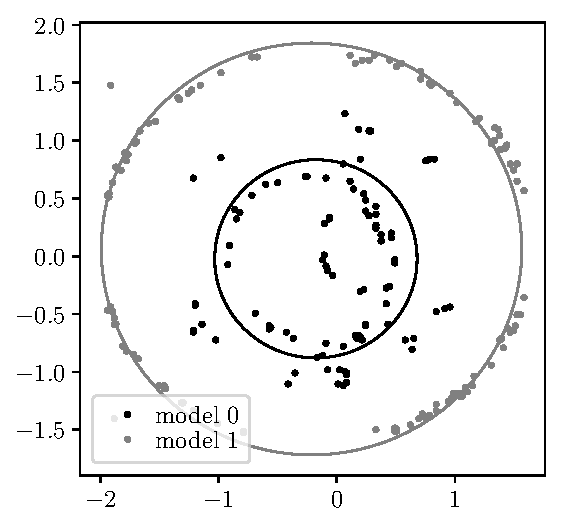
\includegraphics[height = 0.17\textheight]{results/priorexpertfig/prior_real_example}}
	\subfloat[]{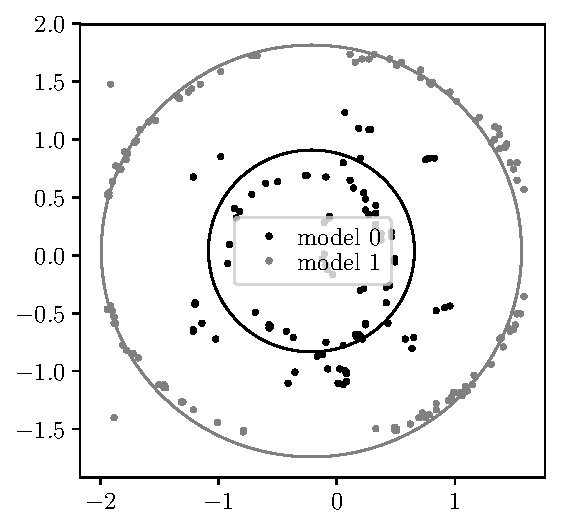
\includegraphics[height = 0.17\textheight]{results/priorexpertfig/prior_regular_real_example}} 
\caption{Визуализация приближения радужной оболочки: а) если указан регуляризатор~$ R_0~$; б) если указан регуляризатор~$ R_1~$; б) если указан регуляризатор~$ R_2~$}
\label{ch4-ce:fig6}
\end{figure}


\begin{figure}
\center
     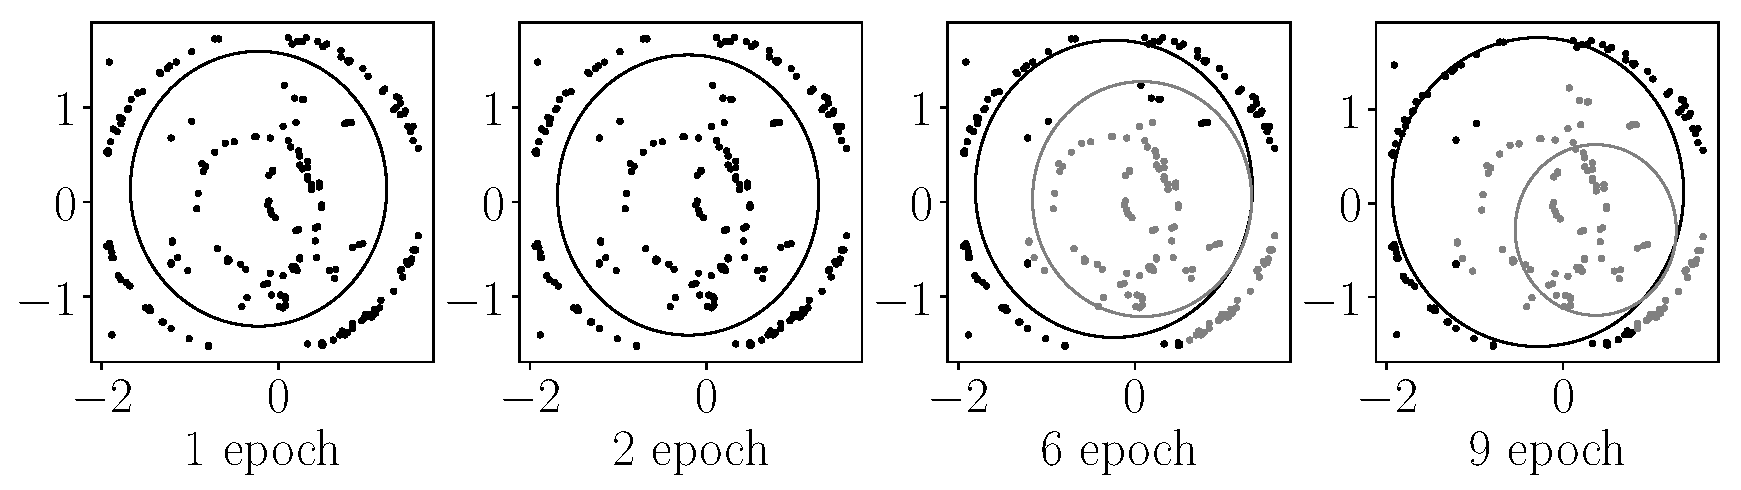
\includegraphics[width=\textwidth]{results/priorexpertfig/experiment_real_not_prior}\\
     \caption{Визуализация процесса сходимости параметров мультимодели в случае регуляризатора~$ R_0~$}
    \label{ch4-ce:fig7}
\end{figure}

\begin{figure}
\center
     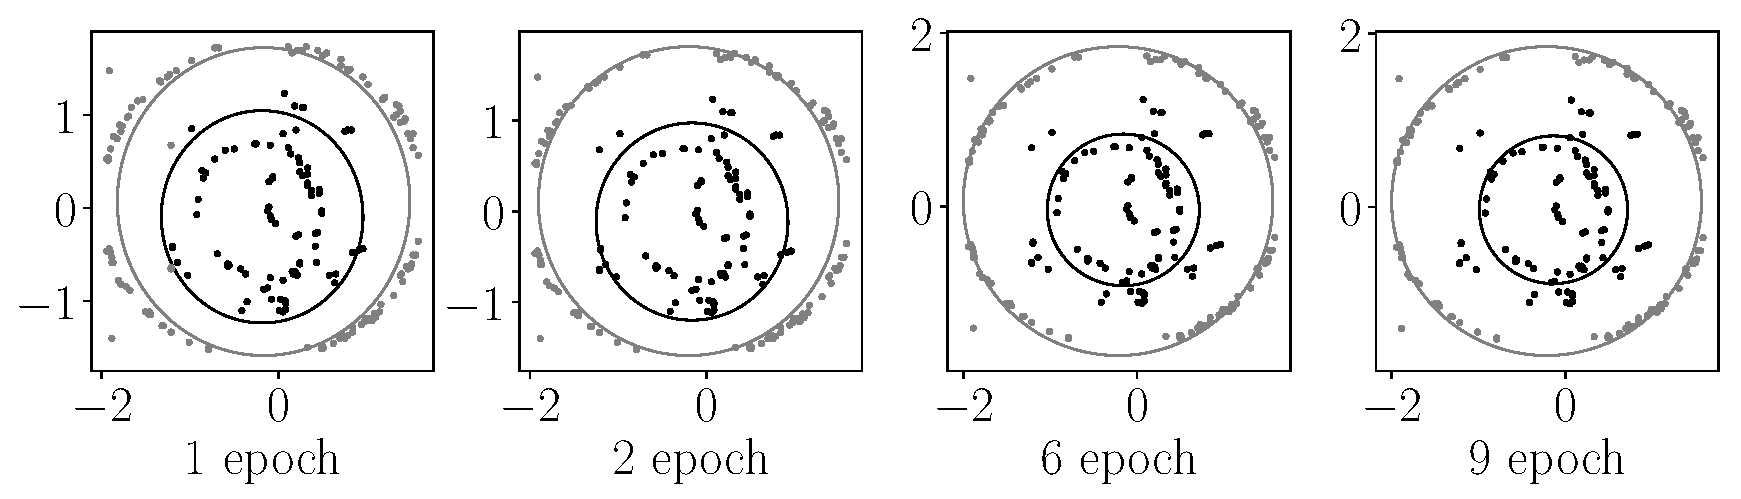
\includegraphics[width=\textwidth]{results/priorexpertfig/experiment_real_prior}
     \caption{Визуализация процесса сходимости параметров мультимодели в случае регуляризатора~$ R_1~$}
    \label{ch4-ce:fig8}
\end{figure}

\begin{figure}
\center
     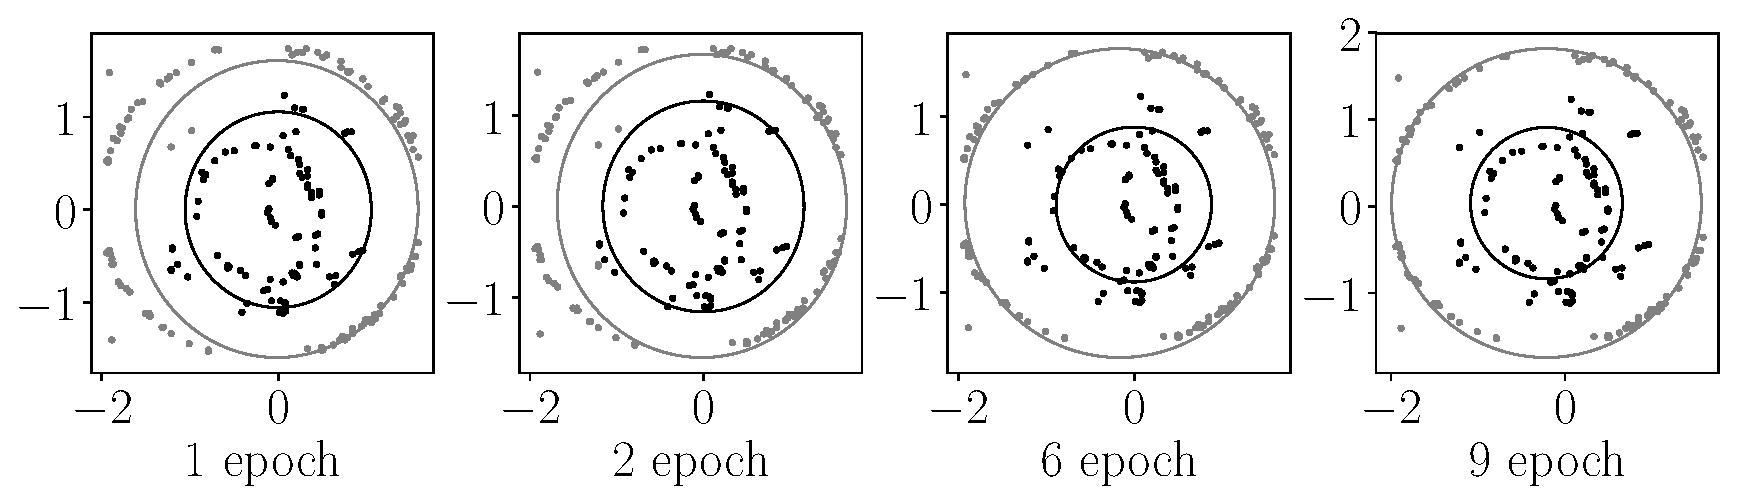
\includegraphics[width=\textwidth]{results/priorexpertfig/experiment_real_regular}
     \caption{Визуализация процесса сходимости параметров мультимодели в случае регуляризатора~$ R_2~$}
    \label{ch4-ce:fig9}
\end{figure}

Анализ качества аппроксимации проводится для задачи аппроксимации радужной оболочки глаза на изображении. Радужная оболочка глаза состоит из двух концентрических окружностей, поэтому рассматривается мультимодель, состоящая из двух экспертов: каждый эксперт аппроксимирует одно из обстоятельств. В вычислительном эксперименте сравнивается качество аппроксимации окружностей при задании разных регуляризаторов~$ R_0, R_1, R_2~$. Регуляризатор~$ R_0 \bigl(\mathbf{V}, \mathbf{W}, E(\Omega) \bigr) = 0,~$ то есть регуляризатора нет. Регуляризатор

\[
R_1\bigl(\mathbf{V}, \mathbf{W}, E(\Omega)\bigr)= -\sum_{k=1}^{K}\mathbf{w}_k^{\mathsf{T}}\mathbf{w}_k,
\]
удаляет околонулевые параметры локальных моделей.
Регуляризатор
\[
R_2\bigl(\mathbf{V}, \mathbf{W}, E(\Omega)\bigr)= -\sum_{k=1}^{K}\mathbf{w}_k^{\mathsf{T}}\mathbf{w}_k + \sum_{k=1}^{K}\sum_{k'=1}^{K}\sum_{j=1}^2\left(w_k^j-w_k'^j\right)^2
\]
способствует совпадению центров окружностей и близким к нулю параметрам модели.
На рисунке \ref{ch4-ce:fig6} показан результат алгоритма аппроксимации радужной оболочки глаза после 10 итераций. Видно, что при отсутствии регуляризатора одна из окружностей находится некорректно. Если задан регуляризатор~$ R_1~$, модель аппроксимирует обе окружности с хорошим качеством, но окружности не концентрические. В случае задания регуляризатора~$ R_2~$ мы получим концентрические окружности на изображении.

На рисунках \ref{ch4-ce:fig7}-\ref{ch4-ce:fig9} показан процесс сходимости мультимоделей в случае задания разных регуляризаторов~$ R_0, R_1, R_2~$. Видно, что модели с типом регуляризатора~$ R_1~$ и~$ R_2~$ аппроксимируют обе окружности, а мультимодель с регуляризатором~$ R_0~$ аппроксимирует только большую окружность.
